\documentclass[
    a4paper,
    man,
    spanish
]{apa6}
\usepackage{booktabs}
\usepackage[spanish,es-tabla]{babel}
\usepackage[utf8]{inputenc}
\usepackage{graphicx}
\usepackage{epstopdf}
\usepackage{csquotes}
\usepackage[hidelinks]{hyperref}
\usepackage[skip=10pt plus1pt, indent=40pt]{parskip}
\usepackage{float}
\usepackage{ragged2e}
\usepackage[
    style=apa,
    backend=biber,
    sorting=nyt,
    hyperref=false,
    backref=false,
]{biblatex}
\usepackage{adjustbox}
\usepackage{multirow}

\usepackage{graphicx}

\usepackage[table,xcdraw]{xcolor}
\DeclareLanguageMapping{spanish}{spanish-apa}

% maps apacite commands to biblatex commands
\let\citeNP\cite\let \citeA\textcite\let\cite\parencite 

%%%
% Apa Bib - enable reprint according to apa
%%%

\bibliography{bibliography}


%%%%%%%%%%%%%%%%%%%%%%%%%%%%%%%%%%%%%%%%%%%%%%%%%%%

\title{Plan de negocio de asistente digital de reseñas y recomendaciones turísticas para nómadas digitales en territorio bogotano }
\shorttitle{Plan de Negocios}

\keywords{emprendimiento, plataforma web, perfilacion, ingeniería web}

\begin{document}


\begin{titlepage}
    \begin{center}
        \vspace*{0.5cm}
            
        \Large
        \textbf{ Plan de negocios de asistente digital de reseñas y recomendaciones turísticas para nómadas digitales en Bogotá }
            
        \vspace{0.5cm}
        \large
        Caso de estudio: Nómadas Digitales 
        
        \vspace{2.5cm}
            
        \normalsize
        \textbf{Jeferson David Nieto Gaona 20202020020}\\
        \textbf{Andrés Felipe Bejarano Baron 20202020055}
            
        \vfill
            
        Proyecto de Emprendimiento para Optar por el Título de\\
        Ingeniero  de Sistemas
            
        \vspace{0.8cm}
            
        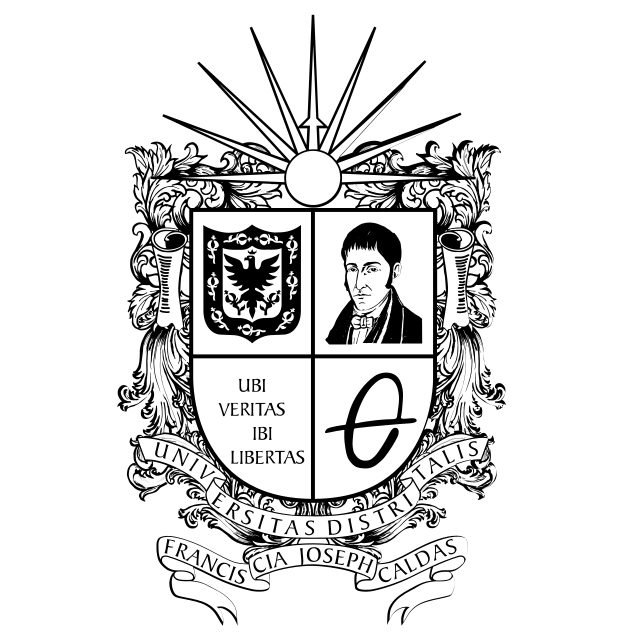
\includegraphics[width=0.2\textwidth]{Content/Images/Escudo_UD.png}
            
        \large
        Universidad Distrital Francisco José De Caldas\\
        Facultad de Ingeniería\\
        Colombia, Bogotá D.C.\\
        Agosto de 2023\\

        
            
    \end{center}
\end{titlepage}

\newpage
\tableofcontents
\newpage
\listoffigures
\newpage
\listoftables
\newpage

\justifying
\raggedbottom 

%-------------RESUMEN---------------------%


\section{Resumen}
\noindent
El propósito del siguiente documento es presentar y justificar el plan de negocio para el desarrollo de una plataforma de reseñas y recomendaciones personalizadas enfocadas a los nómadas digitales en la ciudad de Bogotá. Haciendo énfasis en la seguridad y la comodidad de los usuarios, proporcionando recomendaciones personalizadas basadas en gustos personales, reseñas de usuarios y estudios de seguridad en la zona.

Se implementó la metodología Canvas para estructurar el plan de negocio, definiendo así la propuesta de valor, los segmentos de clientes, los canales de distribución, las fuentes de ingresos y los recursos clave necesarios para el desarrollo de la plataforma. Esta metodología permitió identificar de manera clara los elementos fundamentales para la viabilidad y sostenibilidad del proyecto.
Esto apoyado en el análisis de la matriz DOFA y PEYEA, permitiendo evaluar los ámbitos internos y externos, planteando estrategias que permitan acelerar y garantizar el progreso del proyecto. Además, se realizó el análisis financiero que justifica la viabilidad del proyecto.

Adicionalmente, se identificaron oportunidades de crecimiento y diferenciación frente a la competencia mediante la integración de tecnologías innovadoras y la personalización de los servicios ofrecidos. Se espera que la plataforma sea un referente en el mercado turístico y de tecnología, por su seguridad, fiabilidad y enfoque en la excelente experiencia de usuario.

%-------------INTRODUCCIÓN---------------------%

\section{Introducción}
Bogotá, por su posición geográfica y las 122 mil hectáreas de suelo rural, goza de una invaluable riqueza natural debido a la confluencia de ecosistemas de todo tipo, pues es posible encontrar cerros, llanuras, bosques, humedales, producciones agropecuarias, centros poblados, lagunas, parques y senderos, pudiendo combinar un turismo de naturaleza con montaña, humedales y corredores ecológicos~\cite{EstudioTurismoenterritoriosruralesdeBogotá}.

Para el desarrollo de las actividades de turismo en territorio bogotano es importante comprender a profundidad el panorama de las personas que promueven o realizan esta actividad, dado que es un campo que presenta tanta variedad y riqueza, que tiene ofertas y modalidades que pasan desapercibidas para potenciales consumidores.

Bajo este marco, la nueva ruralidad permite desarrollar una amplia variedad de actividades, empoderando a las comunidades rurales a través de mayores oportunidades de empleo, destacando a los jóvenes y mujeres, favoreciendo la preservación de los hábitats y la conservación del patrimonio natural y cultural de las regiones~\cite{EstudioTurismoenterritoriosruralesdeBogotá}.

Comprendiendo el marco rural de la ciudad, se debe hacer énfasis también en el mercado hotelero y gastronómico, ya que actualmente existen aplicaciones y sitios web con opciones y lugares prometedores para explotar el turismo bogotano. Pese a estas herramientas tecnológicas, la comodidad del usuario final como consumidor o prestador de servicio que quiere darse a conocer no es muy cercana u honesta, ya que muchas plataformas tergiversan las reseñas y manipulan fácilmente a los usuarios finales, influyendo negativamente en su experiencia final.

Es imperativo crear una plataforma que permita dar a conocer el mercado turístico tanto rural como urbano de la ciudad y reseñarlas de forma honesta y transparente.


%-------------PROBLEMA---------------------%

\section{Planteamiento del problema}
Una gran cantidad de turistas al momento de hacer reservas o consultar actividades enriquecedoras para conocer el negocio del turismo en Bogotá caen bajo recomendaciones o fácilmente manipulables ya que empresas poco escrupulosas ofrecen aumentar las reseñas en los sitios web de empresas de hoteles y turismo que no cumplen con los estándares que prometen, pero por sus reseñas sesgadas atraen a clientes bajo engaños y exageraciones. 

Considerando la problemática anteriormente mencionada nace la oportunidad de negocio de crear una herramienta digital en formato de asistente digital que permita reseñas adecuadas, personalizadas, honestas y justificadas, se asegura normalizando que las reseñas tengan evidencias fotográficas o de vídeo de su experiencia positiva o negativa sobre un lugar, así como votar y comentar sobre las opiniones de otra persona para que las reseñas manipuladas no ponderen la evaluación de emprendimientos frecuentados.  

Esta modalidad si bien no garantiza a totalidad que los emprendimientos locales puedan hacerse pasar por consumidores frecuentes para inflar positivamente sus reseñas, podrá hacer más evidente este tipo de manipulación y dar visibilidad de esto al usuario como aviso de que este establecimiento está intentando manipular sus métricas hacia los consumidores y de esta misma forma darle más visibilidad a las reseñas que sean clasificadas y votadas como verdaderas de acuerdo a su respaldo fotográfico o de video. 
\begin{adjustbox}{
    center,
    caption=[{Arbol de problemas}]{\centering Arbol de problemas. Fuente:Autores},
    label={arbol de problemas},
    nofloat=figure}

    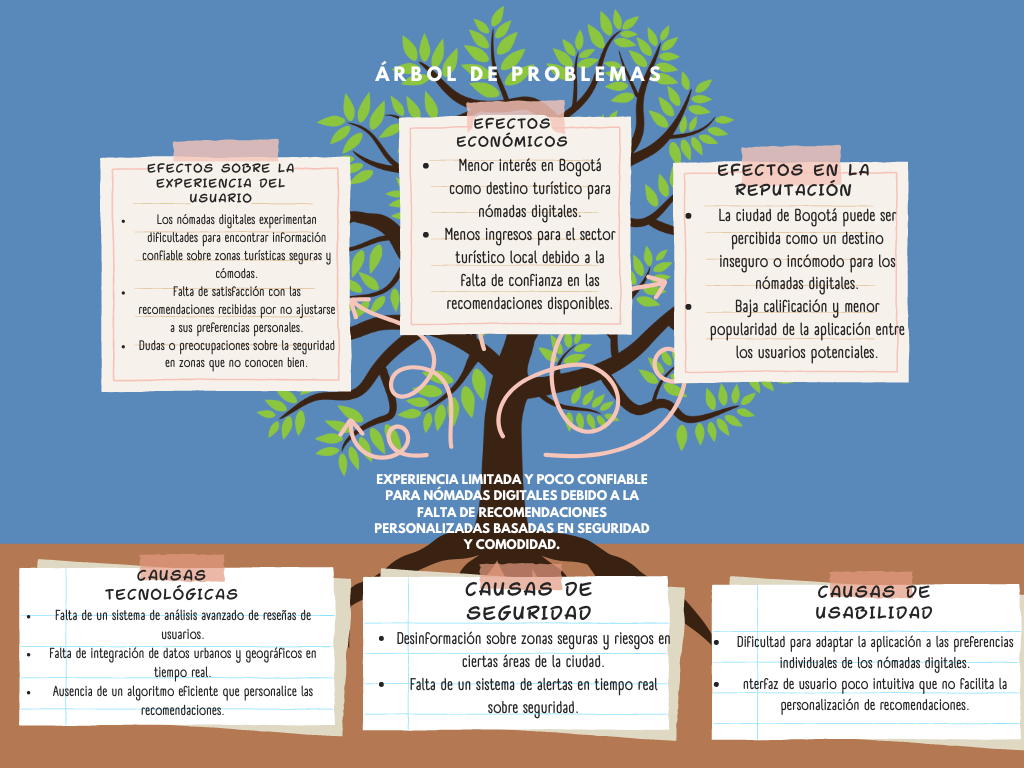
\includegraphics[scale= 0.6]{Content/Images/Gráfica Árbol de problemas emprendimiento (1).png}


\end{adjustbox}


\subsection{Descripción del Problema}
Varias compañías del sector de la restauración–Partoo, Superpopi, Healthy Poke, Talent Class y Localboss– se han posicionado públicamente en contra del filtrado de reseñas. Lo consideran como una manipulación que ofrece una visión distorsionada de la realidad a los consumidores. El año pasado, Google eliminó 170 millones de reseñas y 12 millones de perfiles de empresa que no cumplían con su política de contenido, lo que supone un 43\% más que en 2022, según ha contado recientemente la compañía en su blog.\cite{hotelesReseñasNeg}

Esta declaración deja al descubierto como muchas empresas a sabiendas de que es mas fácil modificar deshonestamente sus reseñas haciéndose pasar por clientes conocedores en el tema del turismo que arreglar sus establecimientos y mejorar sus servicios para que cumplan con las expectativas que le plantean en su publicidad.  

Por el otro lado, otra problemática que también se planea mitigar a nivel local con esta oportunidad de desarrollo es la desmeritar reseñas y opiniones que estén fuera de lugar o estén sesgadas negativamente, entiéndase como una “reseña sesgada negativamente” aquella que no abarca una calificación correspondiente a los productos, servicios o experiencia general del cliente ofrecido directamente por una compañía, por ejemplo, no es justo para el emprendedor local que su negocio sea negativamente calificado porque la tienda de al lado hace ruido o el día que estaba consumando su estadía hubo lluvias y no fue de su agrado, este tipo de reseñas perjudica de sobremanera a un establecimiento y esto se evidencia en trabajos de investigación como el realizado por la revista digital Partoo donde se entrevistó a consumidores sobre su frecuencia a revisar reseñas y se llega a la conclusión de que “El 75\% de los encuestados admite que nunca elige un establecimiento con una valoración inferior a 3.5/5” 

\subsection{Formulación del Problema}
¿Cómo aumentar la confianza de los consumidores de aplicaciones digitales de turismo que ha sido afectada por reseñas sesgadas o calificaciones de reseñas manipuladas? 

\subsection{Justificacion del problema}
Después de la rápida caída del sector del turístico a nivel mundial por causa de la pandemia del 2020, Colombia ha tenido una mejora prometedora a partir del 2022 que inclusive ha impulsado notoriamente el desarrollo de este sector aún más que antes de la pandemia. Esta afirmación está respaldada por los datos estadísticos que la Cámara de Comercio de Bogotá puede ofrecer sobre el sector turístico y su desempeño desde principios de 2019 hasta julio de 2024. Para entender el siguiente gráfico es necesario comprender que el éxito del sector del turismo se mide respecto al porcentaje de cupos que ofrecen para sus actividades y estadías. 

\begin{adjustbox}{
    center,
    caption=[{Porcentaje de ocupación mensual: Total nacional y Bogotá}]{\centering Ocupación mensual Bogotá. Fuente: (DANE, Encuesta mensual de alojamiento EMA (enero 2019 - abril 2024))},
    label={ocupaciónmensualbogota},
    nofloat=figure}

    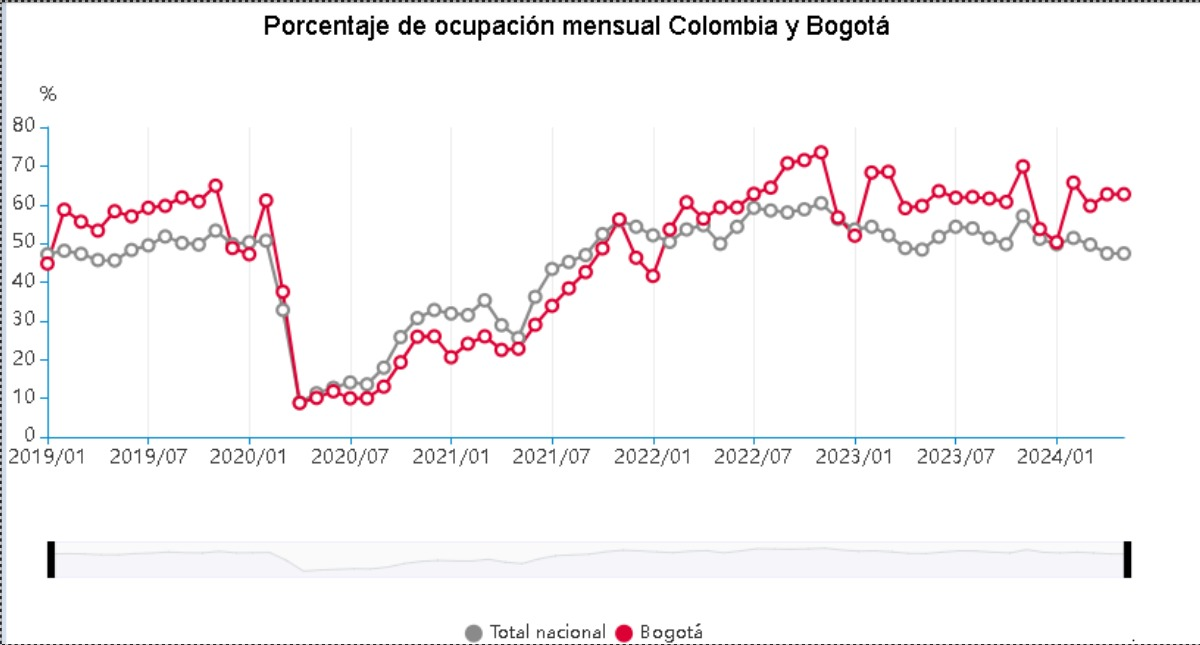
\includegraphics[width=0.2\textwidth]{Content/Images/graficaTurismoBogota.jpeg}

\end{adjustbox}


%-------------OBJETIVOS---------------------%

\section{Objetivos}

\subsection{Objetivo General}

Garantizar recomendaciones seguras y confiables para nómadas digitales que visiten Bogotá, mediante el análisis avanzado de reseñas de usuarios, factores urbanos, geográficos y culturales. La aplicación priorizará la seguridad del usuario al evaluar riesgos en cada destino, considerando niveles de criminalidad, accesibilidad, iluminación y afluencia de personas. Además, ofrecerá opciones que equilibren protección, comodidad y preferencia personal, permitiendo una experiencia turística segura y adaptada a sus necesidades.

\subsection{Objetivos Específicos}
\begin{itemize}
    \item  Desarrollar un sistema de análisis de reseñas de usuarios que permita identificar las preferencias y experiencias previas de los nómadas digitales en diferentes puntos turísticos de la ciudad de Bogotá. 
    \item  Integrar datos urbanos, geográficos y culturales para evaluar y sugerir zonas o actividades que ofrezcan un equilibrio óptimo entre seguridad, accesibilidad, y autenticidad cultural para los usuarios. 
    \item  Crear un perfil personalizado de cada usuario que permita recomendar actividades, zonas o servicios basados en sus preferencias individuales, como el tipo de alojamiento, transporte, espacios de trabajo, y atracciones turísticas.
    \item Implementar un sistema de alerta y recomendación basado en la seguridad que informe a los usuarios sobre las zonas seguras y confortables para trabajar, hospedarse, y disfrutar de su tiempo libre en Bogotá. 
    \item Optimizar la experiencia del usuario mediante la inclusión de sugerencias en tiempo real basadas en cambios en el entorno urbano, como clima, eventos culturales, o cambios en las reseñas más recientes de los puntos turísticos. 
    \item Monitorear y ajustar el algoritmo de recomendación para mejorar la precisión de las sugerencias, ajustándose continuamente a las nuevas reseñas de usuarios y datos dinámicos de la ciudad.

\end{itemize}

%-------------MARCO TEORICO---------------------%


\section{Marco Teórico}

\subsection{Nómada digital}

 Un nómada digital es una persona que utiliza la tecnología para trabajar de forma remota mientras viaja y cambia de ubicación regularmente. Este estilo de vida es posible gracias al acceso a internet, computadoras portátiles y plataformas digitales, lo que les permite a los nómadas digitales trabajar desde cualquier parte del mundo. Los trabajos más comunes entre los nómadas digitales suelen estar en la economía del conocimiento, como diseño, marketing, programación, escritura y consultoría.\cite{NomDig}



\subsection{Metodología ágil}

La metodología ágil es un enfoque para la gestión de proyectos, principalmente en el desarrollo de software, que se caracteriza por su flexibilidad, colaboración continua y respuesta rápida al cambio. Su objetivo es entregar productos funcionales en iteraciones cortas, conocidas como sprints, en lugar de completar todo el proyecto de una sola vez. 

Dentro del marco ágil, hay varias metodologías, como Scrum, Kanban y Extreme Programming (XP). Estas metodologías comparten principios fundamentales, como la entrega de valor al cliente de manera frecuente, la colaboración constante entre los equipos de trabajo y la adaptación continua a los cambios que puedan surgir durante el proceso de desarrollo. \cite{MetAgil}

\subsection{Metodologia Scrum }

Scrum es un marco de trabajo ágil para gestionar proyectos, particularmente en el desarrollo de software, aunque su aplicación se ha expandido a otras áreas. Se basa en principios de colaboración, iteración y entrega incremental de valor. El proceso de Scrum divide el trabajo en ciclos cortos y repetitivos llamados sprints, típicamente de 2 a 4 semanas de duración, durante los cuales los equipos trabajan en alcanzar metas específicas. Al final de cada sprint, se revisa el progreso y se ajustan los objetivos si es necesario.\cite{Scrum}

\subsection{Página web }

Una página web es un documento digital accesible a través de internet, compuesto principalmente de texto, imágenes, videos y enlaces, creado usando lenguajes de marcado como HTML, CSS y JavaScript. Cada página web tiene una dirección única (URL) que permite a los usuarios acceder a ella a través de un navegador web. Las páginas web forman parte de un sitio web, que puede contener varias páginas interrelacionadas. Estas páginas pueden ser estáticas (mostrando siempre el mismo contenido) o dinámicas (modificando su contenido según las interacciones del usuario o de un servidor). \cite{web}


%-------------ALCANCES Y LIMITACIONES---------------------%


\section{Alcances y limitaciones}

\subsection{Alcances}
\begin{itemize}
    \item  Servir como asistente digital para la recomendación de empresas de turismo en consumidores de estos emprendimientos analizando tendencias y experiencias de otros usuarios. 

\item Organizar un sistema de reseñas que donde se regule la transparencia y validez de cada reseña, dándole peso y respaldo a cada una con la inclusión de evidencia fotográfica y de video acerca de los servicios prestados. 

\item Promover la visualización de emprendimientos enfocados hacia la exploración de la cultura en territorio bogotano (Aerolíneas con vuelos a Bogotá, museos, casas de cultura, restaurantes... etc.) 



\end{itemize}


\subsection{Limitaciones }
\begin{itemize}
    \item  Tanto las empresas enfocadas al turismo como sus consumidores están limitados únicamente a territorio bogotano.
    \item Los estudios de mercado son reconocidos a la fecha de presentación de este proyecto ya que son sujetos a posibles fluctuaciones de la moneda nacional y su mercado. 
    \item Este proyecto solo reconocerá emprendimientos que se registren en la aplicación, no todas las empresas de territorio bogotano indiscriminadamente. 
    \item Para registrarse como una empresa proveedora de servicio de turismo debe estar directamente relacionada con la exploración cultural del territorio bogotano, esto acoge a emprendimientos como restaurantes, hoteles y aerolíneas por su estrecha relación con el desarrollo cultural, sin embargo, empresas que sean derivadas de esta exploración cultural no directamente relacionadas no estarán contempladas, tales como emprendimientos de venta de recuerdos, venta de inmuebles o vehículos. 
    \item El proyecto no propone un intermediario entre los consumidores turisticos y las empresas proveedoras de turismo, esto implica que no se recibirá dinero de los consumidores para comprar, organizar o reservar directamente en la empresa de turismo ya que se escapa de las funciones de asistente digital. 
    \item Pese a que se reconoce que la publicidad paga de empresas proveedoras de turismo impulsa su visibilidad frente a los posibles consumidores de sus servicios, esta visibilidad mantiene la filosofía transparente del proyecto y es en su mayoría meritocrática, esto implica que a pesar de que una empresa pague por aumentar su visibilidad, esto no implicará que se muestre por encima de empresas que tengan mejor calidad en la prestacion de sus servicios o productos. Se entiende entonces que esta publicidad paga es un impulso a su visibilidad mas no una garantía de ser los primeros en ser mostrados cuando se presenten opciones a los consumidores turísticos. 





\end{itemize}



%-------------MODELO DE NEGOCIO---------------------%


\section{Modelo de Negocio}
Para el desarrollo del modelo de negocio se implementó el modelo canva , el cual permite visualizar los aspectos fundamentales del modelo de negoccio del proyecto, estos son los socios claves que tendrá la empresa, actividades claves que realizará la empresa, propuestas de valor que tendrá la empresa, recursos clave para llevar a cabo las actividades, la estructurá de costos que manejará la empresa, las relaciones con el cliente que mantendrá la empresa, los canales por los cuales se moverá la empresa, las fuentes de ingresos que tendrá la empresa y los segmentos de clientes que tendrá la empresa.
Lo anteríor mencionado se ve ilustrado en la siguiente figura del modelo canva del proyecto
\begin{adjustbox}{
    center,
    caption=[{Modelo de negocio Canvas}]{\centering Modelo Canvas. Fuente:(Autores)},
    label={Modelo de negocio canvas},
    nofloat=figure}

    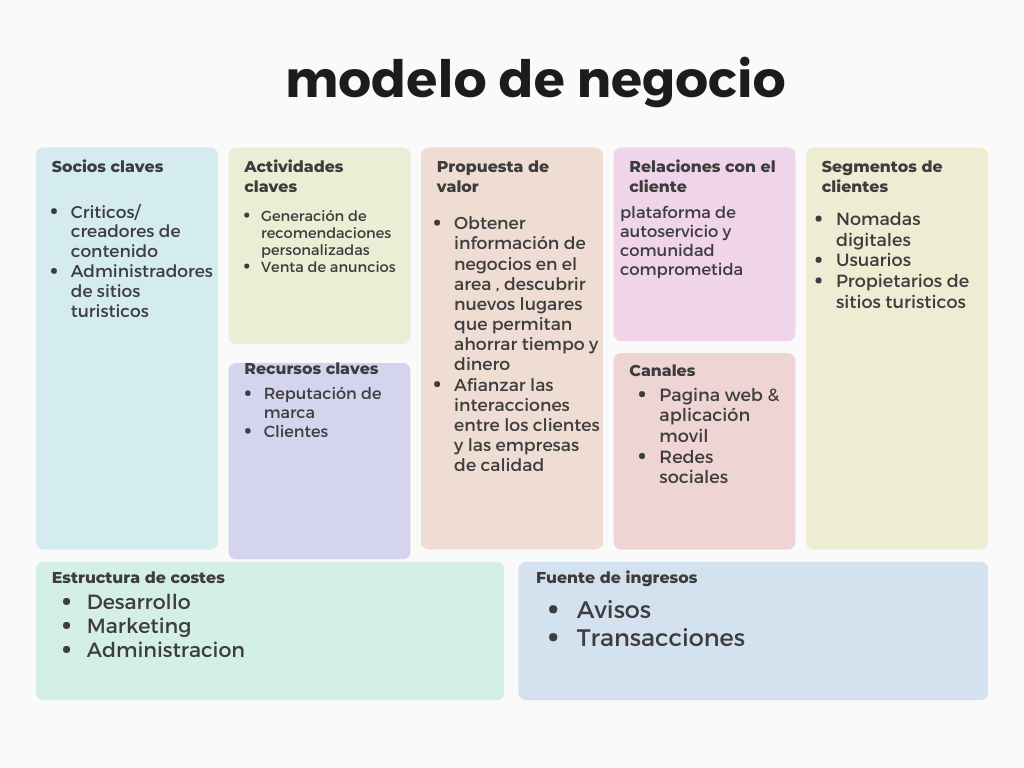
\includegraphics [scale=0.61]{Content/Images/Canva Emprendimiento.png}

\end{adjustbox}


\subsection{Segmento de clientes (SC)}
En esta sección se explora el segmento de clientes al que está enfocado el proyecto, en este caso los segmentos son los nomadas digitales en primer lugar, luego los usuarios generales del proyeto y por ultimo los propietarios de sitios turisticos que deseen ser parte del proyecto promocionandose.
\subsection{Propuesta de valor (PV)}
En esta sección se describen las propuestas de valor que permitirá el proyecto destacar entre los diferentes proveedores del mismo servicio, las propuestas de valor son la obtención de información de negocios en el area,descubrir nuevos lugares que permitan ahorrar dinero y tiempo al usuario final de la aplicación; Además de afianzar las interacciones entre los usuarios y las empresas que demuestren tener un servicio destacable.
\subsection{Canales de distribución (CD)}
En esta sección se especifican los canales de distribución del servicio que dará el proyecto , el principal es la pagina web y la aplicación movil en la que se desplegarán los servicios del proyecto, tambien se tienen en cuenta las redes sociales por ser el canal por el cual se publicitará el proyecto
\subsection{Relaciones con clientes (RCI)}
En esta sección se indican las relaciones que se tendrá con los clientes en la cual se explica que dicha relación será como una plataforma de autoservicio y comunidad comprometida para enriquecer la experiencia de los demás usuarios
\subsection{Fuentes de ingresos (FI)}
En esa sección están las fuentes de ingresos que tendrá el proyecto , las cuales son los avisos de diversos proveedores de servicios de turismo y transacciones al comprar cupones u ofertas que tengan los proveedores de servicios de turismo
\subsection{Recursos clave (RC)}
En esta sección se valoran los recursos clave del proyecto siendo estos la reputación de la marca ya que es fundamental que los usuarios tengan plena confianza en las recomendaciones brindadas, además de este los clientes son clave para que las recomendaciones esten bien fundamentadas en las experiencias de estos.
\subsection{Actividades clave (AC)}
En esta sección se presentan las actividades claves que tendrá el proyecto, estas son la generación de recomendaciones personalizadas, estas se basarán en la ubicación del usuario, en su presupuesto, en las calificaciones de otros usuarios y en las calificaciones pasadas del mismo usuario; además se tendrá la venta de anuncios de proveedores de servicios turisticos , incluso estas estan sujetas a las calificaciones de los usuarios, pero la venta de anuncios les permitirá a los proveedores darse a conocer
\subsection{Asociaciones o socios clave(AsC)}
En esta sección se posicionan los socios clave, comprendiendo a los criticos o creadores de contenido que permitirán dar a conocer el proyecto y esto enriquecerá el banco de recomendaciones mejorando así la calidad de las recomendaciones; tambien se tienen en cuenta los administradores de sitios turisticos ya que estos podrán promocionarse en el proyecto y asi mismo contribuir a aumentar la cantidad de usuarios.
\subsection{Estructura de costos (EC)}
En esta sección se indica la estructura de costes, donde destaca el desarrollo del proyecto, el marketing que se trabajará en el proyecto y la administración del proyecto.

\section{Esquema de ventas}
Un esquema de ventas es la estrategia estructurada que define cómo una empresa comercializa y vende sus productos o servicios. Este esquema establece los canales de distribución, el público objetivo, los procesos de captación de clientes, las fuentes de ingresos y las estrategias de conversión y fidelización.

En otras palabras, el esquema de ventas detalla cómo la empresa genera ingresos mediante un enfoque claro y organizado, asegurando que sus productos o servicios lleguen de manera efectiva a los clientes potenciales.

\subsection{Elementos clave de un esquema de ventas:}
\begin{itemize}
   \item Segmentación del mercado: Identificación de clientes ideales.

\item Propuesta de valor: Beneficio único del producto o servicio.

\item Fuentes de ingresos: Métodos de monetización.

\item Canales de ventas: Medios para atraer y cerrar ventas (online/offline).

\item Estrategias de conversión: Métodos para transformar clientes potenciales en compradores.

\item Fidelización del cliente: Acciones para mantener y retener clientes.
\end{itemize}


\subsection{Esquema de ventas aplicado}

\begin{itemize}
    \item Segmentación del mercado:
    \begin{itemize}
        \item Nómadas digitales que buscan destinos seguros y confiables.
    \item Turistas extranjeros y nacionales interesados en experiencias seguras.
    \item Empresas turísticas (hoteles, coworkings, restaurantes, agencias de tours) que deseen posicionar sus servicios con un enfoque en seguridad.
    \end{itemize}
    \item Propuesta de valor:
    \begin{itemize}
        \item Plataforma confiable con reseñas verificadas.
        \item Sistema de recomendación basado en IA para sugerencias personalizadas.
        \item Mapeo de zonas seguras y alertas en tiempo real sobre riesgos en ciertas áreas.
    \end{itemize}
    \item Fuentes de ingresos:
    \begin{itemize}
        \item Suscripción Premium para usuarios: Acceso a recomendaciones más detalladas, alertas en tiempo real y funciones avanzadas.
        \item Publicidad y asociaciones con negocios locales: Hoteles, restaurantes y espacios de coworking pagan por visibilidad en la plataforma.
        \item Afiliación con seguros de viaje y transporte seguro: Comisiones por referir usuarios a servicios de movilidad confiables y seguros
         \item Análisis de datos para entidades turísticas:  Reportes sobre tendencias de seguridad y comportamiento de los viajeros
    \end{itemize}
    
   \item Canales de ventas:
    \begin{itemize}
        \item Plataforma web y aplicación móvil.
        \item Marketing digital (SEO, SEM, redes sociales, influencers nómadas).
        \item Alianzas con embajadas y asociaciones de nómadas digitales.
        \item Ferias y eventos de turismo y tecnología.
    \end{itemize}
   \item Estrategia de conversión y fidelización:
    \begin{itemize}
        \item Pruebas gratuitas de funcionalidades premium.
        \item Programas de referidos con incentivos.
        \item Descuentos y beneficios exclusivos para suscriptores.
    \end{itemize}
\end{itemize} 


%-------------METDOLOGÍA---------------------%



\section{Metodología}

En este parte del proyecto se aborda la estructura establecida por Osterwalder Yves en el escrito “Generación de modelos de negocios”\cite{modeloNegocio}, se usa para tratar todas condiciones y requisitos fundamentales en el desarrollo de plan de negocios. 

Las fases y actividades establecidas se distribuyen de la siguiente manera:
\subsubsection{Fase 1: Presentación y compromiso del equipo}


\begin{itemize}
    \item Formación del grupo base.
    \item Formación del grupo de trabajo definitivo.
    \item Identificación de áreas de análisis
    \item Presentación del proyecto, procesos y metodologías.
    \item Documento de presentación aprobado (Anteproyecto).
\end{itemize}

En el cuadro \ref{Fase1} se establecen los objetivos de la fase asociada con la presentación y compromiso del equipo de manera que se puedan proyectar ciertos resultados esperados a través de unas actividades especificas de la fase.

\begin{adjustbox}{
            center,
             caption=[{Descripción de la fase 1}]{\centering Descripción de la fase 1. Fuente: : Autores.},
            label={Fase1},
            nofloat=table, vspace={20px}}
            \resizebox{\textwidth}{!}{
            \begin{tabular}{|c|c|c|c|}
            \hline
            \rowcolor[HTML]{D9EAD3} 
            \multicolumn{1}{|l|}{\cellcolor[HTML]{D9EAD3}\textbf{Fase 1}} &
            \multicolumn{1}{l|}{\cellcolor[HTML]{D9EAD3}\textbf{Objetivos Especificos}} &
            \multicolumn{1}{l|}{\cellcolor[HTML]{D9EAD3}\textbf{Actividades}} &
            \multicolumn{1}{l|}{\cellcolor[HTML]{D9EAD3}\textbf{Resultados Esperados}} \\ \hline
             &  & Conformación del equipo       & \begin{tabular}[c]{@{}c@{}}Tener claro el papel de cada uno\\  de los integrantes del equipo\end{tabular} \\ \cline{3-4} 
            &  & Búsqueda inicial de literatura & Análisis del contexto                                                                                      \\ \cline{3-4} 
        \multirow{-4}{*}{\begin{tabular}[c]{@{}c@{}}Presentación y \\ compromiso del \\ equipo\end{tabular}} &
        \multirow{-4}{*}{\begin{tabular}[c]{@{}c@{}}Dar a conocer los integrantes del equipo\\  e iniciar con el análisis de la situación,\\ planteamiento del problema\\  y proyectarnos trabajando de la mano.\end{tabular}} &
            Definir el planteamiento del problema &
            Definición precisa del problema \\ \hline
            \end{tabular}
            }

        \end{adjustbox}

\subsubsection{Fase 2: Análisis de la situación}
\begin{itemize}
    \item Identificación de la oportunidad de negocio, definición del producto o servicios.
    \item Estudio de mercado.
    \item Análisis de riesgos.
\end{itemize}

En el cuadro \ref{Fase2} se establecen los objetivos de la fase asociada al análisis de la situación de manera que se puedan proyectar ciertos resultados esperados a través de unas actividades especificas de la fase.

\begin{adjustbox}{
            center,
             caption=[{Descripción de la fase 2}]{\centering Descripción de la fase 2. Fuente: : Autores.},
            label={Fase2},
            nofloat=table, vspace={20px}}
            \resizebox{\textwidth}{!}{
            \begin{tabular}{|c|c|c|c|}
\hline
\rowcolor[HTML]{D9EAD3} 
\textbf{Fase 2} &
  \textbf{Objetivos Especificos} &
  \textbf{Actividades} &
  \textbf{Resultados Esperados} \\ \hline
 &
   &
  \begin{tabular}[c]{@{}c@{}}Definir el funcionamiento del\\ mercado de contratacion de personal IT\end{tabular} &
  \begin{tabular}[c]{@{}c@{}}Definición de producto\\  y posibles riesgos\end{tabular} \\ \cline{3-4} 
 &
   &
  Establecer las asociaciones claves &
  Modelo de negocio \\ \cline{3-4} 
 &
   &
   &
  Propuesta de valor \\ \cline{4-4} 
\multirow{-5}{*}{\begin{tabular}[c]{@{}c@{}}Análisis de la \\ situación actual\end{tabular}} &
  \multirow{-5}{*}{\begin{tabular}[c]{@{}c@{}}Realizar un análisis de mercado para\\ definir la factibilidad de creación \\ del producto para la gestion \\ de contratacion de personal IT\end{tabular}} &
  \multirow{-2}{*}{\begin{tabular}[c]{@{}c@{}}Efectuar la estructura \\ de costos\end{tabular}} &
  Estudio de mercado \\ \hline
\end{tabular}
            }

        \end{adjustbox}

\subsubsection{Fase 3: Definición de la empresa}
\begin{itemize}
    \item Identificación de la misión, la visión y el objeto de la empresa.
    \item Modelo de negocio que se abordará.
    \item Estructura organizacional y administrativa
    \item Tipo de sociedad a crear.
\end{itemize}
En el cuadro \ref{Fase3} se establecen los objetivos de la fase asociada con la definición del problema de manera que se puedan proyectar ciertos resultados esperados a través de unas actividades especificas de la fase.
\begin{adjustbox}{
            center,
             caption=[{Descripción de la fase 3}]{\centering Descripción de la fase 3. Fuente: : Autores.},
            label={Fase3},
            nofloat=table, , vspace={20px}}
            \resizebox{\textwidth}{!}{
            \begin{tabular}{|c|c|c|c|}
\hline
\rowcolor[HTML]{D9EAD3} 
\textbf{Fase 3} & \textbf{Objetivos Especificos} & \textbf{Actividades} & \textbf{Resultados Esperados} \\ \hline
                &                                & Definir Misión       &                               \\ \cline{3-3}
                &                                & Definir Visión       &                               \\ \cline{3-3}
                &                                &                      &                               \\
\multirow{-4}{*}{\begin{tabular}[c]{@{}c@{}}Definición de \\ la empresa\end{tabular}} &
  \multirow{-4}{*}{\begin{tabular}[c]{@{}c@{}}Establecer la misión y visión de la\\ empresa al igual que el ecosistema empresarial\end{tabular}} &
  \multirow{-2}{*}{Trazar los valores empresariales} &
  \multirow{-4}{*}{\begin{tabular}[c]{@{}c@{}}Conformación de la\\ \\ empresa con todos sus agregados y sus valores\end{tabular}} \\ \hline
\end{tabular}
            }

        \end{adjustbox}

\subsubsection{Fase 4: Estructuración}
\begin{itemize}
    \item Identificación de debilidades y fortalezas (Análisis interno).
    \item Identificación de las oportunidades y amenazas (Análisis externo).
    \item Identificación de funciones y procesos de negocio de la empresa.
    \item Ingeniería.
    \item Estudio técnico.
    \item Estudio legal.
    \item Plan financiero.
    \item Prototipo
\end{itemize}
En el cuadro \ref{Fase4} se establecen los objetivos de la fase asociada con la estructuración de manera que se puedan proyectar ciertos resultados esperados a través de unas actividades especificas de la fase.
\begin{adjustbox}{
            center,
             caption=[{Descripción de la fase 4}]{\centering Descripción de la fase 4. Fuente: : Autores.},
            label={Fase4},
            nofloat=table, vspace={20px}}
            \resizebox{\textwidth}{!}{
            \begin{tabular}{|c|c|c|c|}
\hline
\rowcolor[HTML]{D9EAD3} 
\textbf{Fase 4} & \textbf{Objetivos Especificos} & \textbf{Actividades}                          & \textbf{Resultados Esperados}     \\ \hline
                &                                & Definir presupuesto                           &                                   \\ \cline{3-3}
                &                                & Definir inversión inicial, ingresos y egresos & \multirow{-2}{*}{Estudio técnico} \\ \cline{3-4} 
                &                                & Definir naturaleza jurídica                   &                                   \\ \cline{3-3}
 &
  \multirow{-4}{*}{\begin{tabular}[c]{@{}c@{}}Definir estructura\\ legal del producto\end{tabular}} &
  Establecer propiedad intelectual &
   \\ \cline{2-3}
                &                                & Identificar obligaciones legales              & \multirow{-3}{*}{Estudio legal}   \\ \cline{3-4} 
                &                                & Realizar balance general                      &                                   \\ \cline{3-3}
                &                                & Definir un punto de equilibrio                &                                   \\ \cline{3-3}
                &                                & Análisis de indicadores financieros           &                                   \\ \cline{3-3}
                &                                & Realizar flujo de caja                        & \multirow{-4}{*}{Plan financiero} \\ \cline{3-4} 
                &                                & Realizar estudio del entorno                  &                                   \\ \cline{3-3}
\multirow{-11}{*}{Estructuración} &
  \multirow{-7}{*}{\begin{tabular}[c]{@{}c@{}}Realizar ingenieria \\ del proyecto\end{tabular}} &
  Realizar estado de resultados &
  \multirow{-2}{*}{Estudio ambiental} \\ \hline
\end{tabular}
            }

\end{adjustbox}

\subsection{Cronograma}

Se opta para construir el siguiente cronograma que tiene las actividades propuestas a realizar para el desarrollo exitoso de este proyecto y los tiempos en los que deben llevarse a cabo.

\begin{adjustbox}{
    center,
    caption=[{Cronograma de actividades}]{\centering Cronograma de actividades Fuente: Autores},
    label={Cronograma},
    nofloat=figure, vspace={7px}}


    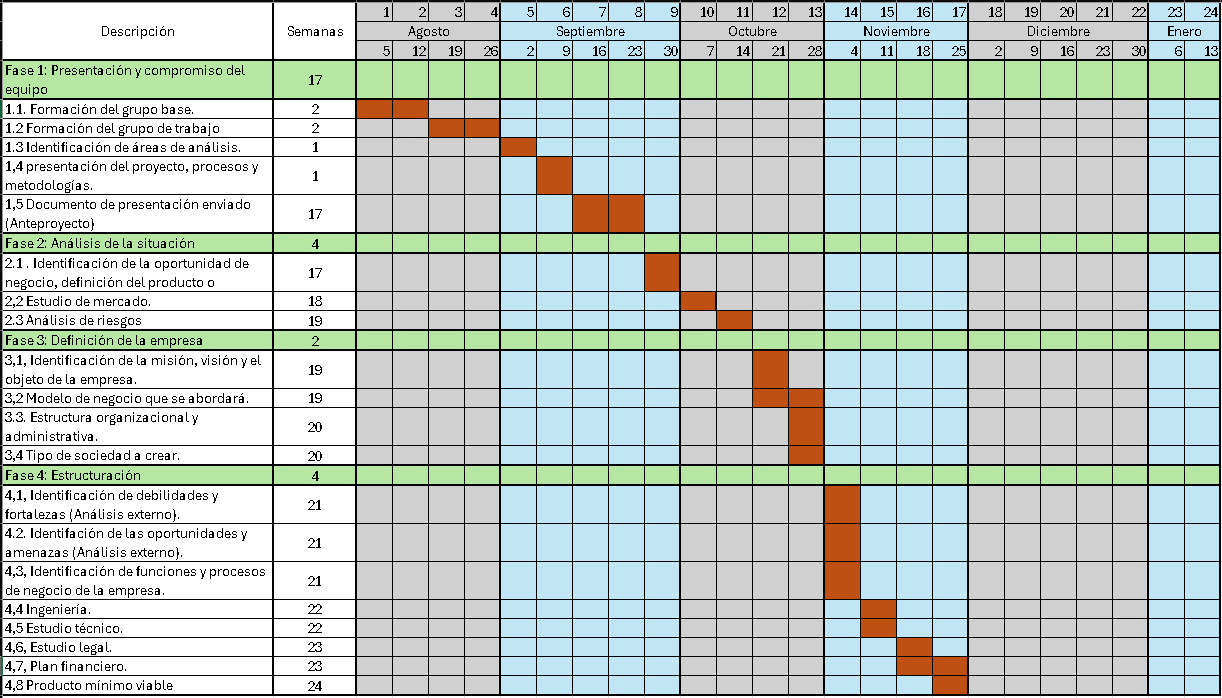
\includegraphics[width=1\textwidth]{Content/Images/cronogramaEmpre.PNG}
\end{adjustbox}






\subsection{Estructura ideológica}

Para este apartado de estructura ideológica se aclaran las creencias y valores publicamente expresados que fundamentan la empresa, para esto se utilizan apartados de:

\begin{itemize}
    \item Se debe definir el nombre de la empresa, una descripción concisa de la misma y el porqué de la elección del nombre. El nombre debe ser atractivo, fácil de recordar y reflejar la esencia del negocio. 
    
    \item Incluye el porqué está creada la empresa, su razón de ser y como su filosofía está plasmada en su funcionamiento.
    \item Visión: Aquí se habla de como se ve la empresa a futuro y como su proyección ha mejorado su esquema de funcionamiento
    \item Valores: Este apartado define las reglas que rigen la organización, incluyendo su relación con los clientes, empleados y la sociedad en general.
    \item Ventajas competitivas: Se mencionan los aspectos que diferencian a la empresa de la competencia, como la calidad del producto, el servicio al cliente, la innovación, entre otros.
    
\end{itemize}




{
    \color{orange}   \subsection{Entorno}
}
{\color{blue}\subsection{Entorno}


En este pilar se consolida la organización en el mercado, realizando el análisis del entorno, integrado por la competencia, aliados y los potenciales clientes.

\begin{itemize}
    \item Matriz DOFA: Metodología diseñada para proporcionar información sobre la situación de la empresa en el mercado, identificando cuatro aspectos clave: Debilidades, Oportunidades, Fortalezas y Amenazas.
    \item Descripción del publico objetivo: Ofrece la presentación y análisis de la población destinataria de la propuesta de valor de la empresa, utilizando estadísticas pertinentes para centralizar la información.
    \item Investigación demográfica del mercado: Se examina el crecimiento del mercado desde un periodo específico hasta el presente, considerando el estado actual del mercado y proyectando su desarrollo a corto, mediano y largo plazo.
    \item Frecuencia de adquisición del producto: Establece un método para calcular un índice que determine la frecuencia esperada con la que los clientes potenciales puedan adquirir el producto ofrecido, obteniendo proyecciones con un margen de error mínimo.
    \item Estudio de la competencia: Basado en el benchmarking, se analizan las ideas y pilares de cada entidad competidora, centrándose en el valor agregado y las estrategias de mercadotecnia utilizadas.
\end{itemize}
}

\subsection{Estructura mecánica}

En esta sección se describe la fase productiva, basandose en los objetivos planteados junto con el plan de acción de la empresa.Su finalidad es ejecutar la estrategia comercial y de mercadeo para garantizar ingresos regulares y sostenibles.

\begin{itemize}
    \item Precio del servicio: Se establece el costo del producto o servicio, garantizando que sea equilibrado con los gastos y ganancias de la empresa. También se analizan los precios de la competencia para mantener una tarifa competitiva.
    
    \item Planes de pago: Se detallan las formas de pago aceptadas, promociones iniciales, descuentos especiales y facilidades de crédito o financiamiento para los clientes.

    \item Fuerza en ventas:Se define la cantidad de personal necesario para desarrollar operaciones, junto con sus características y capacidades clave para promover el producto eficazmente. También se establecen sus salarios, comisiones y beneficios.

    \item Canales de distribución: Se explican las rutas o métodos utilizados para hacer llegar el producto o servicio a los consumidores finales.
    
    \item Canales de comunicación:Se seleccionan las herramientas y plataformas para informar, atraer y mantener contacto con clientes actuales, potenciales y el público en general.
\end{itemize}



\subsection{Estructura financiera}
Esta sección tiene como finalidad proporcionar información fundamental del plan de negocio en la cual se refleja la viabilidad del proyecto fundamentada en el estudio financiero del proyecto. Esta se basa en 6 pilares.
\begin{itemize}
    \item Estado de resultado pro-forma proyectado a tres años:Es una proyección del comportamiento financiero de la empresa en el futuro,estimando ingresos,costos,gastos y utilidades basados en supuestos realistas.Esto con la finalidad de prever rentabilidad y planificar estrategias operativas o de inversión.
    \item Balance general proyectado a cinco años:Refleja a situación financiera de la empresa(activo,pasivos y patrimonios)a cinco años.Los activos siendo efectivo,inventario y propiedades.Los pasivos siendo deudas a corto/largo plazo.El patrimonio siendo capital social y utilidades acumuladas.Este balance permite evaluar la solvencia y la capacidad de crecimiento de la empresa a futuro.
    \item Flujo de caja pro-forma proyectado a cinco años:Se realiza un pronostico de entradas y salidas de efectivo ya sea en operaciones financieras,inversiones o financiamientos durante cinco años, esto con la finalidad de identificar necesidades de liquidez, capacidad para pagar deudas y evitar crisis de efectivo.
    \item Análisis del punto de equilibrio: Es el cálculo del volumen de ventas necesario para cubrir costos totales(fijos y variables) donde las utlidades son cero.Esto con la finalidad de determinar la viabilidad de un negocio y fijar metas mínimas de ventas.
\end{itemize} 





\subsection{Recursos humanos}
Es un área encargada de gestionar el talento humano, desde su reclutamiento hasta su desarrollo y retención.Sus funciones clave son la selección donde se contrata el personal idóneo para el puesto ofertado,capacitación donde se forman y desarrollan habilidades para desempeñar el cargo asignado,Administración donde se gestionan nóminas,beneficios y leyes laborales acordes al puesto y contrato del empleado,Clima laboral donde se fomenta un entorno de trabajo positivo. Todo esto con la finalidad de alinear las necesidades de la empresa con el bienestar y productividad de los empleados.



%-------------INFORMACION DE LA EMPRESA---------------------%

\section{Información de la empresa}

\subsection{Misión}

\textcolor{red}{El proyecto se dedica a potenciar la vitalidad y el bienestar de los nómadas digitales a través de servicios de fitness personalizados y experiencias de bienestar integradas en la cultura y el espacio urbano de Bogotá. Se compromete a proporcionar soluciones innovadoras y accesibles que fomenten un estilo de vida activo, fortalezcan la salud mental y física, y creen una comunidad de individuos conscientes y conectados, no importando dónde se encuentren.}

\subsection{Visión}
\textcolor{red}{La visión del proyecto es ser la plataforma líder en bienestar y fitness para nómadas digitales, reconocida por su enfoque personalizado y su capacidad para adaptarse a los estilos de vida móviles. Aspira a transformar la salud y el ejercicio en una experiencia cultural enriquecedora, expandiéndose más allá de Bogotá para llegar a ser una referencia global en bienestar, y al mismo tiempo, un agente de cambio social y ambiental positivo.}

\subsection{Valores}

\begin{itemize}
    \item \textbf{Innovación:} \textcolor{red}{Adaptamos continuamente nuestra plataforma y servicios para ofrecer soluciones de vanguardia en entrenamiento y bienestar, respondiendo proactivamente a las tendencias emergentes en un mundo globalizado.}
    \item \textbf{Mejora continua:} \textcolor{red}{Comprometidos con la excelencia, evaluamos y perfeccionamos constantemente cada aspecto de nuestra operación, buscando la eficiencia y eficacia en nuestro servicio.}
    \item \textbf{Inclusión:} \textcolor{red}{Promovemos un entorno que valora y respeta la diversidad, proporcionando servicios que liberan el potencial de cada individuo y fomentan la inclusión en todos los niveles.}
    \item \textbf{Competitividad:} \textcolor{red}{Nos enfocamos en el crecimiento sostenible invirtiendo en las mejores oportunidades y talento, con el fin de destacar en el mercado y ofrecer el mejor servicio a nuestros usuarios.}
    \item \textbf{Orientación a objetivos:} \textcolor{red}{Nuestra gestión está enfocada en el logro de resultados, actuando con responsabilidad y cumpliendo con nuestros compromisos para garantizar la satisfacción y el éxito de nuestros clientes.}
    \item \textbf{Colaboración:} \textcolor{red}{Priorizamos la colaboración y el trabajo en equipo, compartiendo conocimientos y experiencias para lograr objetivos comunes y avanzar juntos hacia nuestro propósito colectivo.}
\end{itemize}


\subsection{Modelo organizacional}
\vspace{2mm}
        \begin{minipage}{0.9\textwidth}
        \centering
        \captionof{figure}[{Modelo Organizacional}]{ Modelo Organizacional.  }
        \label{ModeloOrganizacional}
         \includegraphics[width=0.9\textwidth]{Images/orga.png}
        \fnote{Nota. \textup{Fuente: Autores.}}
\end{minipage}



%-------------PLAN DE NEGOCIO---------------------%


\section{Plan de negocio}

\subsection{Estudio de mercado}
\subsection*{Identificación del producto}
El producto es una plataforma enfocada en la comodidad y seguridad de los nomadas digitales en Bogotá que buscan un lugar seguro y de calidad para vivir y trabajar. La plataforma ofrece información sobre la seguridad de las zonas de la ciudad, recomendaciones de lugares que se acoplan al perfil del usuario basandonos en analisis de gustos y experiencias, así como una comunidad de apoyo para los nómadas digitales.

La plataforma ofrece las siguientes funcionalidades:
\begin{itemize}
    \item Registro de usuario: Los usuarios pueden registrarse y acceder con su usuario y contraseña para disfrutar de todas las funciones que el sistema brinda.
    
    \item Evaluación integral de seguridad: Analiza en tiempo real factores como niveles de criminalidad, iluminación, afluencia de personas y accesibilidad, combinando datos oficiales con inteligencia artificial
    \item Recomendaciones personalizadas: Basadas en el perfil del usuario, preferencias y experiencias previas, la plataforma sugiere zonas y lugares que se alinean con sus necesidades.
    \item Ecosistema colaborativo: Una comunidad de apoyo para los nómadas digitales,compartiendo espacios nomad-friendly(Ej: zonas de coworking 24/7, lugares con buena conexión a internet, etc).
\end{itemize}

\subsection*{Demanda}
El proyecto satisface la creciente demanda de nómadas digitales y profesionales remotos en Bogotá que buscan un lugar seguro y de calidad para vivir y trabajar, valorando la seguridad y la comodidad en su entorno.Además de empresas globales que envian talento remoto a Bogotá y requieren garantizar la seguridad de sus empleados.

\subsection*{Oferta}
Comprendiendo la demanda mencionada, se debe analizar la oferta existente en el mercado para identificar las ventajas competitivas de la plataforma. Estas ventajas se traducen en un valor agregado significativo para los usuarios, como:
\begin{itemize}
    \item Una experiencia de usuario personalizada que integra la seguridad y la comodidad en un solo lugar, facilitando la vida diaria de los nómadas digitales.
    
    \item Una interfaz que no solo permite a los usuarios gestionar su seguridad, sino también descubrir y conectarse con otros nómadas digitales, proporcionando una solución integral para la vida nómada.
    
    \item La función de recomendaciones personalizadas que ofrece sugerencias basadas en las preferencias y el historial de actividad de los usuarios, incentivando la participación en la comunidad local.
\end{itemize}

\subsection*{Plan de marketing}
El marketing estratégico es vital para conectar con nómadas digitales y empresas en Bogotá, posicionándose como la plataforma líder en seguridad verificada. Estas acciones no solo generarán reconocimiento local, sino que sentarán las bases para su expansión internacional, construyendo una base de usuarios leales y una marca confiable en el ecosistema nómada.
\textbf{Objetivos}
\begin{itemize}
    \item Lanzar la plataforma destacando su propuesta única de seguridad inteligente para nómadas digitales en Bogotá, con recomendaciones validadas y actualizadas en tiempo real.
    \item Lograr una adopción rápida entre nómadas y empresas mediante campañas digitales segmentadas y alianzas con espacios nomad-friendly.
    \item Fidelizar usuarios con alertas personalizadas, contenido útil sobre seguridad urbana y una comunidad colaborativa dentro de la app.
    \item Posicionarse como referente en seguridad para nómadas digitales en Colombia, con proyección a mercados como Medellín.
    \item Maximizar ingresos mediante un modelo freemium, suscripciones premium, alianzas con coworkings y hostales certificados.

\end{itemize}

\textbf{Táctica}
El proyecto implementará un enfoque de inbound marketing,siendo una metodología centrada en atraer, interactuar y deleitar al público objetivo mediante contenido valioso y no intrusivo. Este enfoque es ideal para construir confianza en un mercado donde la seguridad es prioritaria.

\begin{itemize}
    \item \textbf{Enfoque en Contenido de Valor:}Se basa en la creación y distribución de contenido útil (blogs, guías, webinars) diseñado para resolver problemas específicos del público objetivo, sin vender directamente.
    \item \textbf{Atracción Orgánica (No Intrusiva):}Utiliza estrategias como SEO, redes sociales y email marketing para atraer tráfico cualificado que busca activamente soluciones.
    \item \textbf{Segmentación por Buyer Personas:}El contenido se personaliza según las necesidades, etapas del buyer's journey y características demográficas/conductuales de cada segmento.
    \item \textbf{Construcción de Relaciones a Largo Plazo:}Prioriza la fidelización mediante comunidades, soporte continuo y experiencias personalizadas, convirtiendo usuarios en promotores de la marca.
\end{itemize}
El objetivo principal de la metodología inbound marketing es atraer, convertir, cerrar y deleitar a los clientes potenciales mediante estrategias no intrusivas, centradas en ofrecer valor, resolver problemas y construir relaciones a largo plazo. Se diferencia del marketing tradicional al priorizar la educación sobre la venta directa, guiando al público a través de un proceso natural de decisión.

Como se observa en la figura \ref{inboundMarkting-1} se muestran las etapas del inbound marketing que se implementarán en el proyecto, para asegurar el correcto desarrollo de la estrategia de marketing y la satisfacción del cliente.



\vspace{2mm}
        \begin{minipage}{0.9\textwidth}
        \centering
        \captionof{figure}[{Fases Inbound Marketing}]{ Fases Inbound Marketing  }
        \label{inboundMarkting-1}
         \includegraphics[width=0.8\textwidth]{Content/Images/Metodología Inbound-1.jpeg}
        \footnote{Nota. \textup{Fuente: Inbound Marketing, la guía completa \cite{InboundMarketing}}}
\end{minipage}

\begin{itemize}
    \item \textbf{Atraer:}Esta primera etapa se centra en atraer nómadas digitales que busquen una solución a sus problemas encontrando lugares seguros y de calidad para vivir y trabajar. Utilizando estrategias de marketing de contenido, como la creación de contenido útil (guías, blogs, infografías, etc.) orientado a resolver sus necesidades y posicionar la plataforma como referente en seguridad y comodidad para nómadas digitales en Bogotá.
    \item \textbf{Convertir:}Luego de atraer a los nómadas digitales, el objetivo es convertir a los usuarios en leads, es decir, en contactos interesados en la plataforma. Esto ofreciendo recursos descargables como mapas, rutas y demás que puedan ser de interés para el usuario, a cambio de su información de contacto como email, utilizando formularios optimizados.
    \item \textbf{Cerrar:}Una vez que se han convertido en leads, el siguiente paso es cerrar la venta. Esto se logra mediante el uso de herramientas de automatización de marketing y email marketing, Automatizando emails personalizados (ej.: serie de onboarding con tips de seguridad) y contenido relevante para guiar a los leads hacia la decisión de compra. Se utilizarán técnicas de lead scoring para identificar a los leads más calificados y priorizar su seguimiento.
    \item \textbf{Deleitar:}Por ultimo se busca deleitar a los usuarios, convirtiéndolos en promotores de la plataforma. Esto se logra mediante la creación de una comunidad activa y participativa, donde los usuarios puedan compartir sus experiencias, recomendaciones y consejos sobre seguridad y bienestar en Bogotá. Se fomentará la interacción a través de foros y redes sociales, creando un sentido de pertenencia y lealtad hacia la marca.
\end{itemize}

Permitiendo vincularnos mas profundamente con los nómadas digitales y crear una comunidad sólida que respalde la plataforma. Nuestro proyecto les brindará valor y soluciones a sus problemas, generando confianza y lealtad hacia la marca,aumentando el alcance de la misma a base de su fidelidad y confianza.

\subsection*{Precio}
El precio de la plataforma se ha establecido teniendo en cuenta el análisis de la competencia y el valor agregado que ofrece. Se ha realizado un estudio de mercado para determinar el rango de precios de servicios similares en la región, considerando factores como la calidad del servicio, la personalización y la seguridad.
El precio de la plataforma se ha fijado en un rango competitivo. Se espera que el precio sea atractivo para los nómadas digitales y empresas que buscan soluciones de seguridad y bienestar personalizadas, el precio se ha calculado en base a los siguientes factores:

\begin{itemize}
    \item Valor de Seguridad Verificada:Crear un valor agregado único que justifique el precio premium, destacando que el proyecto ofrece datos de seguridad validados en tiempo real por expertos locales, no solo información crowdsourced como la competencia.
    \item Modelo de Monetización Flexible:Asegurar la sostenibilidad financiera mediante un modelo escalable que combine opciones freemium (acceso básico gratuito) con suscripciones premium ($5-$15 USD/mes) para funcionalidades avanzadas como alertas personalizadas.
    \item Benchmarking Competitivo: Analizar exhaustivamente los precios y características de alternativas como NomadList y SafeCity para posicionar a Triavel como la opción más equilibrada entre costo y valor real en seguridad verificada.
    \item Demanda y Disposición a Pagar:Evaluar cuidadosamente la disposición a pagar del mercado objetivo mediante estudios cuantitativos y cualitativos, considerando tanto nómadas individuales como empresas con empleados remotos.
    \item Fidelización mediante Experiencia:Desarrollar programas de lealtad que transformen usuarios ocasionales en clientes recurrentes, ofreciendo beneficios exclusivos como validaciones prioritarias o acceso a eventos comunitarios.
    \item Soporte Técnico como Diferenciador:Incluir en la estructura de precios el costo de ofrecer un soporte técnico excepcional y personalizado, convirtiéndolo en un argumento de venta único frente a competidores con atención automatizada.
\end{itemize}

\begin{adjustbox}{
            center,
            caption=[{Precio en el mercado actual}]{\centering Precio en el mercado actual (Valores en pesos colombianos COP). },
            label={Precio},
            nofloat=table, vspace={20px}}
            {
       \begin{threeparttable}
           \begin{tabular}{|p{11cm}|p{10cm}p{2cm}|}
                \hline
                \rowcolor[HTML]{D9EAD3} 
                \cellcolor[HTML]{D9EAD3}                              & \multicolumn{2}{c|}{\cellcolor[HTML]{D9EAD3}Precio}            \\ \cline{2-3} 
                \rowcolor[HTML]{D9EAD3} 
                 \multirow{-2}{*}{\cellcolor[HTML]{D9EAD3}Suscripción} & \multicolumn{1}{l|}{\cellcolor[HTML]{D9EAD3}Mínimo} & Máximo   \\ \hline
                                \multicolumn{1}{|l|}{Mensualidad}                     & \multicolumn{1}{l|}{\$30000}                       & \$3600000 \\ \hline
                                \multicolumn{1}{|l|}{Anualidad}                       & \multicolumn{1}{l|}{\$360000}                      & \$3600000 \\ \hline      \end{tabular}
            \begin{tablenotes}[para,flushleft]
                \vspace{2mm}
               \textit Nota. Fuente: Autores.
            \end{tablenotes}
            
        \end{threeparttable}
    }

\end{adjustbox}

El precio de la plataforma se ha fijado en un rango competitivo, con una mensualidad que oscila entre \$50.000 y \$300.000 COP, dependiendo de las funcionalidades y servicios adicionales que se ofrezcan. Este rango se ha establecido tras un exhaustivo análisis de la competencia y la identificación de las necesidades del mercado objetivo.
Se tendrá en cuenta la posibilidad de ofrecer diferentes planes de suscripción, que incluyan desde un acceso básico gratuito hasta opciones premium con funcionalidades avanzadas, como alertas personalizadas y validaciones prioritarias. Esto permitirá captar una amplia gama de usuarios, desde nómadas digitales individuales hasta empresas de turismo que buscan expandir sus operaciones en Bogotá, dichas opciones de suscripción se detallan a continuación:

\begin{adjustbox}{
            center,
            caption=[{Precios de suscripción.}]{Precios de suscripción mensual y anual },
            label={PrecioPeriodos},
            nofloat=table, vspace={20px}}
            {
            \begin{threeparttable}
                \begin{tabular}{|p{7cm}|p{4cm}|p{4cm}|}
                    \hline
                    \rowcolor[HTML]{D9EAD3}
                    Suscripción & Mensualidad & Anualidad \\ \hline
                    Plan gratuito & \$0 & \$0 \\ \hline
                    Plan personal premium & \$30.000 & \$360.000 \\ \hline
                    Plan empresarial & \$240.000 & \$2.880.000 \\ \hline
                    Plan empresarial premium & \$300.000 & \$3.600.000 \\ \hline
                \end{tabular}%
                \begin{tablenotes}[para,flushleft]
                    \vspace{2mm}
                    \textit Nota. Fuente: Autores.
                \end{tablenotes}
            \end{threeparttable}
    }
\end{adjustbox}

\subsection{Stakeholders}

{\color{red}
Los stakeholders son las personas, grupos, organizaciones o entidades que tienen un interés o se ven afectados directa o indirectamente por el plan de negocio propuesto, como se evidencia a continuación: 

\begin{itemize}
    \item Clientes o usuarios finales: Personas con interés en salud y fitness que buscan mejorar su condición física o alcanzar objetivos específicos mediante el uso de la herramienta y profesionales ocupados que necesitan flexibilidad horaria. 

    Entre los usuarios meta se encuentran miembros de comunidades fitness como SmartFit o Bodytech y usuarios de gimansios locales en Bogotá.
    
    \item Entrenadores o profesionales del deporte: Entrenadores certificados en disciplinas específicas (pesas, cardio, funcional, etc.), nutricionistas registrados en COLNUD (Colegio Colombiano de Nutricionistas y Dietistas) y fisioterapeutas con experiencia en recuperación deportiva. 

    Los aliados potenciales son entrenadores que trabajan de forma independiente o en cadenas como Bodytech, SmartFit y Action Fitness. 
    
    \item Equipo interno de la empresa: Desarrolladores de software y desarrolladores UX/UI que crean y mantengan la plataforma digital con interfaces amigables que motiven al uso, además de soporte al cliente para la resolución de dudas sobre la plataforma o planes. 

    Pueden ser contratados por medio de plataformas de desarrollo como Workana o Torre o con agencias como que ofrezcan servicios tecnológicos y consultoría. 
    
    \item Socios estratégicos: Centros deportivos o gimnasios locales para promover la plataforma entre sus clientes, así como empresas de tecnología que ofrezcan herramientas de videollamadas y análisis de datos. 

    Entre los socios estratégicos se plantea la promoción cruzada con cadenas como Bodytech, SmartFit, gimnasios locales y pequeñas y medianas empresas que comercien artículos deportivos o suplementos alimenticios.     
    
    \item Inversionistas o financiadores: Financiamiento externo por entidades de crédito o bancarias e inversionistas que aportan capital inicial al desarrollo de la plataforma.     
    
    \item Proveedores de tecnología: Proveedores de hosting y mantenimiento de la plataforma web y plataformas de pago en línea como intermediarios para manejar los pagos de suscripciones. 

    Puede implementarse los servicios de AWS (Amazon Web Services) o Azure en cuanto al almacenamiento y hosting y pasarelas de pago como Mercado Pago, PayU o Epayco para transacciones locales. 

     \item Comunidad de Bogotá: Grupos locales de fitness que puedan promover la plataforma y organizaciones de bienestar que recomienden el servicio como parte de sus programas. 

     Entre las comunidades disponibles se encuentran grupos como Run Bogotá o CrossFit Bogotá, así como alianzas con programas locales como Ciclovía para afianzar la promoción del sitio. 

     \item Entidades gubernamentales y regulatorias: Instituciones de salud y deporte para asegurar que los servicios cumplen con normativas locales y autoridades fiscales y regulatorias para cumplir con los requisitos legales y tributarios. 

     Entre las entidades que respalden el proyecto, se encuentra el Ministerio de Salud y Proyección Social de Colombia, así como la Dirección de Impuestos y Aduanas Nacionales (DIAN) para el cumplimiento de obligaciones fiscales, en cuando al apoyo de la promoción de actividades físicas, el Instituto Distrital de Recreación y Deporte (IDRD). 

\end{itemize}


}

\subsection{Estudio técnico}
\subsection{Tamaño}
Basandose en el enfoque principal del proyecto, siendo este los nomadas digitales en Bogotá, realizando un análisis del mercado y los recursos necesarios para su desarrollo.El crecimiento del proyecto se verá fundamentado en:

\begin{itemize}
    \item \textbf{Estructura operativa agil:}El proyecto se conformará con un equipo de desarrollo, equipo de analisis de datos y un equipo de marketing, que tendrán un crecimiento escalable y sostenible a lo largo del tiempo.Dichos equipos estarán enfocados en la creación de un producto que se adapte a las necesidades del mercado, permitiendo una rápida adaptación a los cambios y tendencias del sector.
    \item \textbf{Oportunidad de mercado:} Hay un constante crecimiento en el recibimiento de nomadas digitales en Bogotá,pero un gran porcentaje de estos reportan la inseguridad como una barrera para su permanencia en la ciudad,destacando de esta manera la necesidad de un servicio que les brinde seguridad y bienestar,grantizando una mejor experiencia en su estancia.
    \item \textbf{Arquitectura tecnologica:} Plataforma desarrollada con herramientas escalables (AWS, IA para análisis de riesgo) y bajo costo operativo, facilitando el crecimiento proyectado sin sacrificar la calidad del servicio ni aumentar la inversion inicial de manera significativa. La plataforma se diseñará para ser flexible y adaptable, asegurando la integración de nuevas funcionalidades y servicios conforme el mercado evolucione.
\end{itemize}

Comprendiendo estos aspectos, se fundamenta la viabilidad del proyecto, además de su crecimiento y desarrollo sostenido. Supliendo las necesidades del mercado de nómadas digitales en Bogotá, que desean una experiencia segura y de calidad durante su estancia en la ciudad.

\subsection*{Localización}
La localización del proyecto es fundamental para garantizar la conexion con el mercado objetivo y la infraestructura necesaria para su desarrollo. En este caso, se considera la ciudad de Bogotá como el lugar ideal para establecer la sede del proyecto, debido a su creciente comunidad de nómadas digitales y la infraestructura tecnológica disponible.
Para tomar esta decisión, se han evaluado diversos factores:
\begin{itemize}
    \item \textbf{Acceso a talento:} Bogotá cuenta con una amplia oferta de profesionales en tecnología, marketing y desarrollo de negocios, lo que facilita la formación de un equipo competente y especializado. La presencia de universidades reconocidas y centros de formación técnica garantiza un flujo constante de talento joven y actualizado en las últimas tendencias del sector. Además, la ciudad atrae a profesionales de otras regiones del país y del extranjero, enriqueciendo la diversidad y capacidades del equipo.

    \item \textbf{Infraestructura tecnológica:} La ciudad dispone de una infraestructura tecnológica avanzada, con acceso a internet de alta velocidad, centros de datos, servicios en la nube y soporte técnico especializado, lo que es esencial para el desarrollo y operación del proyecto. Bogotá también cuenta con zonas tecnológicas y parques empresariales que ofrecen servicios complementarios como seguridad, energía estable y espacios de trabajo colaborativo, facilitando la operación continua y eficiente del emprendimiento.

    \item \textbf{Ecosistema emprendedor:} Bogotá alberga un ecosistema emprendedor en crecimiento, con espacios de coworking, incubadoras y aceleradoras que pueden apoyar el desarrollo del proyecto. Existen múltiples eventos, ferias y programas de networking que fomentan la colaboración y el intercambio de conocimientos entre emprendedores, inversores y expertos del sector. Además, la ciudad ofrece acceso a fondos de inversión, programas de apoyo gubernamental y alianzas estratégicas que potencian el crecimiento y la sostenibilidad de nuevas empresas.
\end{itemize}

\textbf{lugares candidatos:} Considerando los factores mencionados,se han identificado varios lugares en Bogotá que cumplen con los requisitos necesarios para establecer la sede del proyecto. Dichos lugares demuestran tener la infraestructura adecuada, espacios de trabajo colaborativo y acceso a servicios tecnológicos, lo que los convierte en opciones viables para la localización del proyecto.

\begin{itemize}
    \item \textbf{ParqueSoft:} Parquesoft Bogotá es un proveedor multi-sectorial de servicios de Tecnologías de la Información, que funciona con el apoyo de más 50 empresas de base tecnológica en Bogotá, que trabajando juntas generan una oferta de valor integral, creando soluciones de calidad, a la vanguardia con últimas tendencias digitales.Se debe destacar que Parquesoft apoya a empresas emergentes garantizando innovación,pasión y sinergia entre las empresas que allí se encuentran, además de contar con un equipo de profesionales altamente capacitados y comprometidos con el desarrollo tecnológico del país.

\begin{adjustbox}{center, caption={Precios de Espacios en ParqueSoft}, label={ParqueSoftPrecios}, nofloat=table, vspace={20px}}
    \begin{threeparttable}
        \centering
        \begin{tabular}{|p{7cm}|p{8cm}|}  % Definir las columnas de tamaño adecuado
            \hline
            \cellcolor[HTML]{D9EAD3}\textbf{Tipo de Servicio} & \cellcolor[HTML]{D9EAD3}\textbf{Costo Mensual} \\ \hline
            Suscripción Mensual   & \$96.000 - Total Anual: \$1.152.000 \\ \hline
            Suscripción Semestral & \$78.000/Mes - Total Anual: \$932.000 \\ \hline
            Suscripción Anual     & \$69.000/Mes - Total Anual: \$828.000 \\ \hline
        \end{tabular}
        \begin{tablenotes}[para,flushleft]
            \vspace{2mm}
            \textit{Nota. Fuente: ParqueSoft.com}
        \end{tablenotes}
    \end{threeparttable}
\end{adjustbox}

\item \textbf{Decisión:} Realizando una evaluación de las opciones disponibles,Parquesoft demuestra ser el lugar ideal para desarrollar y establecer la sede del proyecto,considerando los precios de los espacios, el enfoque de tecnologia y el apoyo al emprendimiento emergente. Parquesoft ofrece un apoyo integral a las empresas emergentes, permitiendo el correcto desarrollo del proyecto y su posicionamiento en el mercado,manteniendo las bases de innovación,pasión y sinergia.
\end{itemize}

\subsection*{Tipo de emprendiemiento} El proyecto de calatalogará como un Startup,desarrollada bajo la metodologia Lean Startup, ya que esta metodologia se adapta perfectamente a las características del proyecto, permitiendo un enfoque ágil y flexible en el desarrollo del producto. 

La metodología Lean Startup se centra en la creación de un producto mínimo viable (PMV) que permita validar las hipótesis del negocio con una inversión mínima, facilitando la adaptación y evolución del proyecto conforme a las necesidades del mercado.
Esta metodologia permite un enfoque iterativo, donde se construye, mide y aprende de manera continua, lo que es esencial para el desarrollo de un producto innovador y escalable como el propuesto en este proyecto.

La razón de esta metodología es aprender en poco tiempo, invirtiendo los mínimos recursos. Lean Startup es una metodología dirigido a la puesta en marcha de ideas innovadoras, donde no se comienza creando una empresa, sino una Startup, entendida no como una empresa en pequeño, sino como «una institución humana diseñada para crear un nuevo producto o servicio bajo condiciones de incertidumbre extrema» 
\cite{MetodologiaLean}

\begin{minipage}{0.9\textwidth}
        \centering
        \captionof{figure}[{Metodología Lean Startup}]{Ciclo de Desarrollo Lean Startup}
        \label{leanStartUp}
         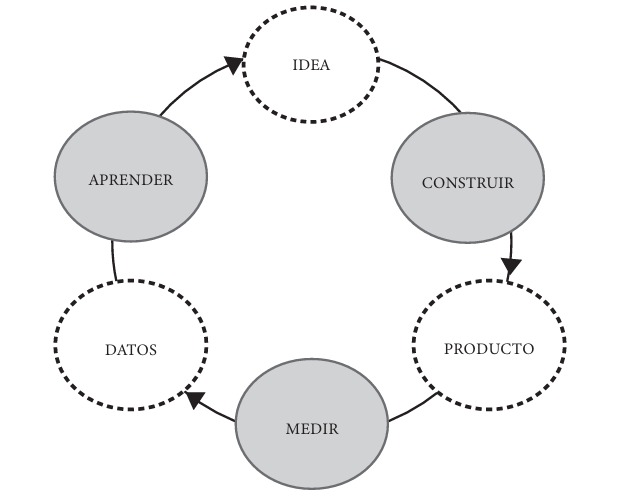
\includegraphics[width=0.7\textwidth]{Content/Images/cicloMetodologiaLean.jpeg}
        \footnote{Nota. \textup{Fuente: Lean Startup, creando productos escalables \cite{GioSyst3m}}}
\end{minipage}

Adoptando esta metodologia el proyecto se desarrollará de manera iterativa, permitiendo demostrar la viabilidad del producto y su aceptación en el mercado, minimizando riesgos y maximizando oportunidades de éxito. Además de permitir una rápida adaptación a los cambios del mercado y a las necesidades de los clientes, lo que es esencial para el éxito de un proyecto innovador como el propuesto.

La selección final del lugar se basará en un análisis detallado de los beneficios, costos y oportunidades que cada opción ofrece, con el objetivo de maximizar el impacto del proyecto tanto en línea como en el entorno local.

\subsection{Equipo de trabajo}
El equipo de trabajo esta compuesto por profesionales altamente capacitados y con capacidades transversales, aportando un gran apoyo al desarrollo del proyecto. El equipo se conforma por:
\begin{itemize}
    \item \textbf{Gerente General / CEO:} Lidera la estrategia global, gestión de recursos y expansión del proyecto, asegurando su posicionamiento como referente en seguridad para nómadas digitales.
    
    \item \textbf{Líder de Tecnología (CTO):} Dirige el desarrollo de la plataforma, enfocandose en la buena experiencia del usuario y la escalabilidad de la misma.
    
    \item \textbf{Director de Operaciones } Supervisa la red de recomendaciones , el algoritmo de evaluación de riesgos y las alianzas con entidades que presten servicios al publico deseado,Con la finalidad de evolucionar continuamente el proyecto basandose en los objetivos y estrategias planteadas.
\end{itemize}
\begin{adjustbox}{
            center,
            caption=[{Equipo de trabajo.}]{Equipo de trabajo. },
            label={EquipoDeTrabajo},
            nofloat=table, vspace={20px}}
            \resizebox{\textwidth}{!}{
            \begin{threeparttable}
            \begin{tabular}{|cllll|cllll|}
            \hline
            \multicolumn{5}{|c|}{\cellcolor[HTML]{D9EAD3}Integrante} & \multicolumn{5}{c|}{\cellcolor[HTML]{D9EAD3}Rol}                                          \\ \hline
            \multicolumn{5}{|c|}{Andrés Felipe Bejarano Barón}        & \multicolumn{5}{c|}{Gerente general, líder de la área de ingeniería}                      \\ \hline
            \multicolumn{5}{|c|}{Jeferson David Nieto Gaona}   & \multicolumn{5}{c|}{Directora del departamento de investigación, desarrollo e innovación} \\ \hline
            \end{tabular}%
            
            \begin{tablenotes}[para,flushleft]
                \vspace{2mm}
                \textit Nota. Fuente : Autores.
            \end{tablenotes}
            \end{threeparttable} 
            }    
    \end{adjustbox}


\subsection{Prototipo mínimo viable}
El proyecto tiene como finalidad desarrollar una página web que ofrezca recomendaciones confiables y enfocadas en la seguridad y comodidad de los nómadas digitales que se encuentran en Bogotá. El desarrollo se llevará a cabo usando arquitecturas y herramientas que den pie a la creación de una plataforma sostenible, escalable y adaptada a las necesidades de los usuarios, priorizando la experiencia del usuario a través de la seguridad y confianza en la información que se le brinda.

\textbf{Tecnologías}
\begin{itemize}
    \item \textbf{Spring Boot: } Spring Boot es un framework de desarrollo de aplicaciones Java que simplifica la creación de aplicaciones empresariales. Proporciona una configuración automática y una amplia gama de herramientas para facilitar el desarrollo, lo que permite a los desarrolladores centrarse en la lógica del negocio en lugar de la configuración del entorno.
    Spring Boot es especialmente útil para crear aplicaciones web y servicios RESTful, ya que incluye características como la gestión de dependencias, la configuración de seguridad y la integración con bases de datos. Además, permite el despliegue rápido de aplicaciones en entornos de producción, lo que lo convierte en una opción popular para el desarrollo ágil.
    \vspace{2mm}
    \begin{minipage}{0.9\textwidth}
        \centering
        \captionof{figure}[{Logo Spring Boot}]{Logo Spring Boot}
        \label{Firestore}
         
\includegraphics[width=0.3\textwidth]{Content/Images/spring-boot-logo.png}
        \footnote{Nota. \textup{Fuente: spring.io}}
    \end{minipage}

    \item \textbf{Angular: } Angular es un framework web que permite a los desarrolladores crear aplicaciones rápidas y fiables.
    Mantenido por un equipo dedicado de Google, Angular ofrece un amplio conjunto de herramientas, API y bibliotecas para simplificar y optimizar el flujo de trabajo de desarrollo. Angular ofrece una plataforma sólida para crear aplicaciones rápidas y fiables que escalan con el tamaño de tu equipo y de tu código fuente.

    Angular es muy útil para el desarrollo de aplicaciones web modernas, ya que permite crear interfaces de usuario dinámicas y reactivas. Su enfoque basado en componentes facilita la reutilización del código y mejora la mantenibilidad de las aplicaciones. Además, Angular cuenta con un ecosistema robusto que incluye herramientas para pruebas, enrutamiento y gestión del estado, lo que lo convierte en una opción popular para el desarrollo de aplicaciones empresariales.
    
    \vspace{2mm}
    \begin{minipage}{0.9\textwidth}
        \centering
        \captionof{figure}[{Logo Angular}]{Logo Angular}
        \label{angularLogo}
        
\includegraphics[width=0.25\textwidth]{Content/Images/angular-logo.png}
        \footnote{Nota. \textup{Fuente: angular.io}}
    \end{minipage}
    
    \item \textbf{PostgreSQL: } PostgreSQL es un potente sistema de base de datos relacional de objetos de código abierto con más de 35 años de desarrollo activo, lo que le ha valido una sólida reputación de confiabilidad, robustez de características y rendimiento.

    La comunidad de código abierto proporciona muchos lugares útiles para familiarizarse con PostgreSQL, incluyendo la documentación oficial, tutoriales y foros de discusión. PostgreSQL es conocido por su capacidad para manejar grandes volúmenes de datos y transacciones complejas, lo que lo convierte en una opción popular para aplicaciones empresariales y sistemas de gestión de datos críticos.
    \vspace{2mm}
    \begin{minipage}{0.9\textwidth}
        \centering
        \captionof{figure}[{Logo PostgreSQL}]{Logo PostgreSQL}
        \label{postgresqlLogo}
        
\includegraphics[width=0.3\textwidth]{Content/Images/postgresql-logo.png}
        \footnote{Nota. \textup{Fuente: postgresql.org}}
    \end{minipage}

    \item \textbf{Inteligencias artificiales:} En el desarrollo de este proyecto, se contempló la integración de diversas inteligencias artificiales para mejorar la experiencia del usuario y optimizar el rendimiento de la plataforma. Estas IA se utilizarán para analizar datos, personalizar recomendaciones y mejorar la seguridad del sistema. Algunas de las aplicaciones específicas incluyen:
        \begin{itemize}
            \item \textbf{Análisis de datos: } Utilizar IA para procesar y analizar grandes volúmenes de datos, identificando patrones y tendencias que pueden ser útiles para los usuarios. Para esto se emplea NLP (Natural Language Processing) para el análisis de reseñas y comentarios de los usuarios, permitiendo una comprensión más profunda de las necesidades y preferencias de los nómadas digitales.
            \item \textbf{Recomendaciones personalizadas: } Implementar embeddings, los cuales permiten capturar relaciones semánticas y contextuales entre palabras para ofrecer recomendaciones personalizadas basadas en las preferencias y comportamientos de los usuarios, mejorando la relevancia de las sugerencias de lugares y servicios, además de permitir recomendaciones explicables y fundamentadas.
            \item \textbf{Seguridad: } Emplear IA para detectar y prevenir amenazas de seguridad, mejorando la protección de los datos sensibles de los usuarios, además de la detección de fraudes y actividades sospechosas en la plataforma, haciendo análisis de datos de usuarios sospechosos.
        \end{itemize}
\end{itemize}
\vspace{5mm}
\textbf{Arquitectura} 

\begin{itemize}
    \item\textbf{Arquitectura de microservicios: } Los microservicios son una arquitectura de software donde la aplicación se divide en pequeños servicios independientes, cada uno con una función específica (ej.: autenticación, procesamiento de pagos, geolocalización), que se comunican entre sí mediante APIs. A diferencia de las aplicaciones monolíticas, cada microservicio puede desarrollarse, desplegarse y escalarse por separado, usando tecnologías distintas según su necesidad.
        Esta arquitectura permite escalar selectivamente funciones críticas (como alertas en tiempo real o validación de zonas), integrar tecnologías diversas y aislar fallos sin colapsar todo el sistema. Además, facilita la expansión modular a nuevas ciudades y optimiza costos en la nube al escalar solo lo necesario.
        \vspace{2mm}
        \begin{center}
        \begin{minipage}{0.9\textwidth}
            \centering
            \captionof{figure}[{Arquitectura de Microservicios.}]{Ejemplo de arquitectura de microservicios.}
            \label{microservicios}
            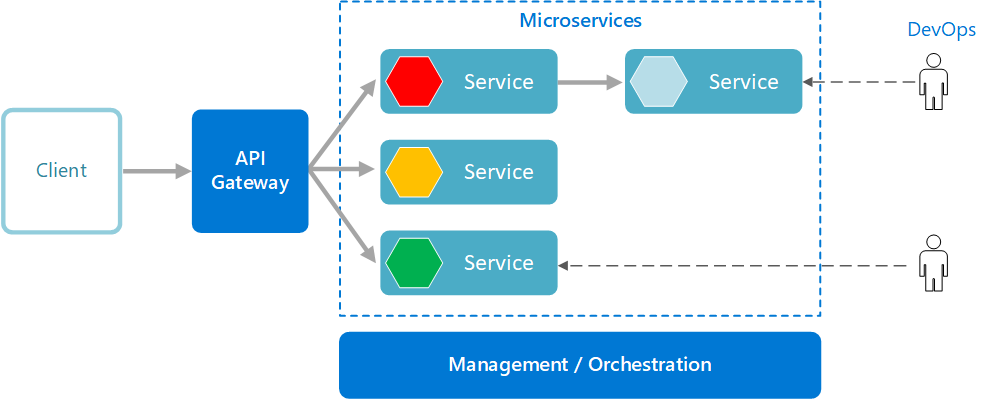
\includegraphics[width=0.9\textwidth]{Content/Images/microservices-logical.png}
            \footnote{Nota. \textup{Fuente: learn.microsoft.com/es-es/azure/architecture/guide/architecture-styles/microservices}}
        \end{minipage}
        \end{center}
    \item \textbf{Arquitectura hexagonal: } La arquitectura hexagonal, también llamada arquitectura de puertos y adaptadores, es un enfoque propuesto por Alistair Cockburn que estructura el software en capas para separar claramente las funcionalidades. Su objetivo principal es mantener el núcleo del sistema (el dominio) aislado, permitiendo que las interacciones con servicios externos (como bases de datos o APIs) se realicen a través de adaptadores específicos.

Gracias a esta separación, los distintos componentes del sistema pueden evolucionar y mantenerse de forma independiente, lo que facilita tanto la escalabilidad como la integración de nuevas tecnologías o servicios. En este modelo, el dominio central permanece protegido de los cambios externos, mientras que los adaptadores gestionan la comunicación con el entorno.
Al hacer uso de esta arquitectura, se tienen diversos beneficios y ventajas con respecto a otras arquitecturas, como los despliegues independientes donde cada componente, tales como análisis de reseñas, monitorización de alertas, validación de zonas, entre otros, pueden ser desplegados, actualizados o revertir cambios sin necesidad de poner offline toda la aplicación. 
Se tiene la facilidad de poder escalar cada componente de forma independiente, lo que permite que la aplicación pueda crecer y adaptarse componente por componente, optimizando costos y recursos. También se tiene la capacidad de cumplir con estándares de manejo de datos sensibles como cifrado reforzado sin complicar el resto de la plataforma. Además, se facilita la integración de nuevas tecnologías o servicios, ya que los adaptadores permiten conectar el núcleo del sistema con diferentes fuentes de datos o APIs sin afectar la lógica central.

    \vspace{2mm}
    \begin{minipage}{0.9\textwidth}
        \centering
        \captionof{figure}[{Arquitectura Hexagonal.}]{Ejemplo de arquitectura hexagonal.}
        \label{hexagonal}
        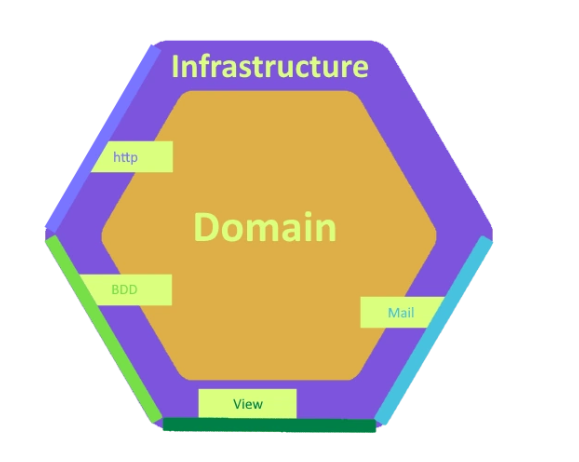
\includegraphics[width=0.9\textwidth]{Content/Images/hexagonal.png}
        \footnote{Nota. \textup{Fuente: https://softwarecrafters.io/react/arquitectura-hexagonal-frontend}}
    \end{minipage}
\vspace{2mm}
\begin{minipage}{0.9\textwidth}
    \centering
    \captionof{figure}[{Arquitectura Hexagonal.}]{Ejemplo de arquitectura hexagonal.}
    \label{hexagonal}
    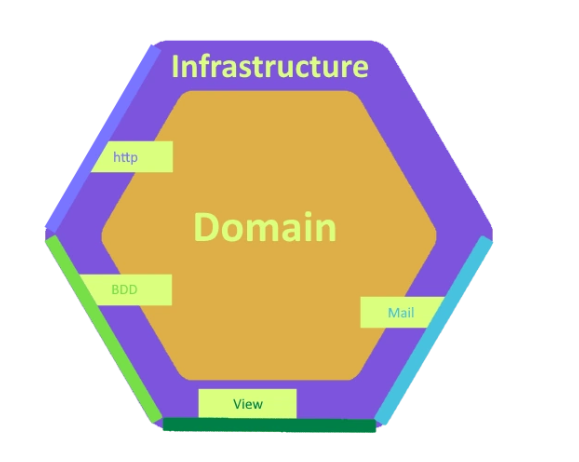
\includegraphics[width=0.5\textwidth]{Content/Images/hexagonal.png}
    \footnote{Nota. \textup{Fuente: https://softwarecrafters.io/react/arquitectura-hexagonal-frontend}}
\end{minipage}
    
\end{itemize}
\textbf{Infraestructura}
\newline
La computación en la nube constituye un pilar esencial para este proyecto, ya que posibilita el acceso y la provisión de almacenamiento, servidores, aplicaciones y otros recursos a través de Internet bajo un modelo de pago por uso. En vez de depender de infraestructuras físicas o centros de datos locales, se recurre a servicios remotos y gestionados, lo que facilita la escalabilidad y optimiza la administración de los recursos.

En este contexto, se ha optado por AWS Lightsail como plataforma en la nube. AWS Lightsail proporciona una infraestructura sencilla y rentable que facilita tanto el desarrollo como el despliegue de aplicaciones, ofreciendo servicios como servidores virtuales, almacenamiento, bases de datos y gestión de redes, todo desde una única plataforma. Esto elimina la necesidad de gestionar servidores físicos o realizar configuraciones complejas, permitiendo que el equipo de desarrollo se concentre en la creación de la aplicación. 
\newline
\textbf{Software as a Service (SaaS):}
El modelo SaaS (Software como Servicio) es ampliamente utilizado en este proyecto, ya que AWS Lightsail permite implementar soluciones bajo este enfoque. Al tratarse de un servicio gestionado, Lightsail permite a los desarrolladores enfocarse en el desarrollo del software sin preocuparse por la administración de servidores físicos, actualizaciones de seguridad o gestión de licencias. Los usuarios pueden acceder a la aplicación y sus funcionalidades desde cualquier lugar con conexión a Internet, lo que simplifica tanto el uso como la operación del sistema. 

\textbf{Requisitos}

\begin{enumerate}
    \item Funcionales
        \par\vspace{2mm}
        \begin{minipage}{0.9\textwidth}
        \centering
        \captionof{table}[{Requisitos funcionales.}]{Requisitos funcionales.}
        \label{req1}
        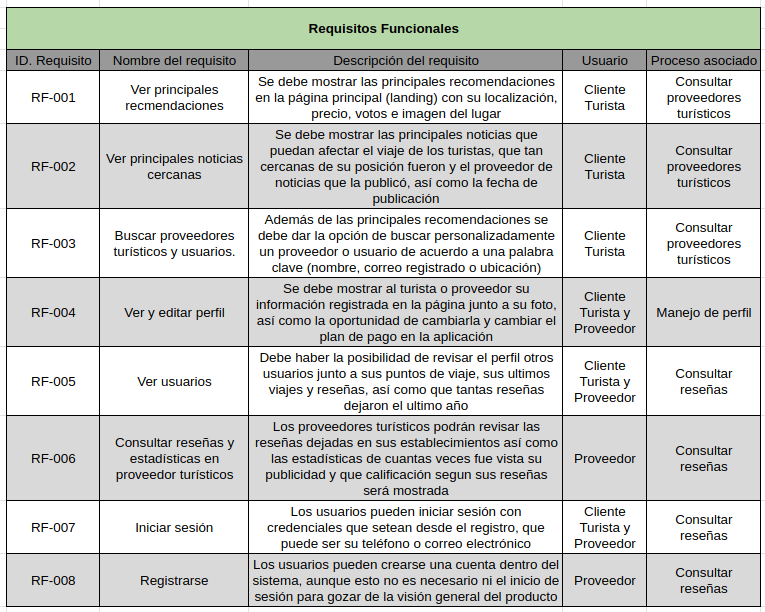
\includegraphics[width=1\textwidth]{Content/Images/requisitos.png}
        \footnote{}{Nota. \textup{Fuente : Autores.}}
        \end{minipage}
           
    \item No funcionales
    \par\vspace{2mm}
        \begin{minipage}{0.9\textwidth}
        \centering
        \captionof{table}[{Requisitos no funcionales.}]{Requisitos no funcionales.}
        \label{req1}
        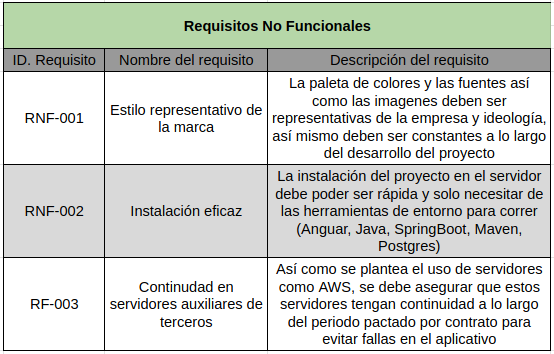
\includegraphics[width=1\textwidth]{Content/Images/requisitosNF.png}
        \footnote{}{Nota. \textup{Fuente : Autores.}}
        \end{minipage}
        
\end{enumerate}

\textbf{Casos de uso}

    \vspace{2mm}
    \begin{minipage}{0.9\textwidth}
    \centering
    \captionof{figure}[{Diagramas de caso de uso.}]{Diagramas de caso de uso.}
    \label{caso1}
    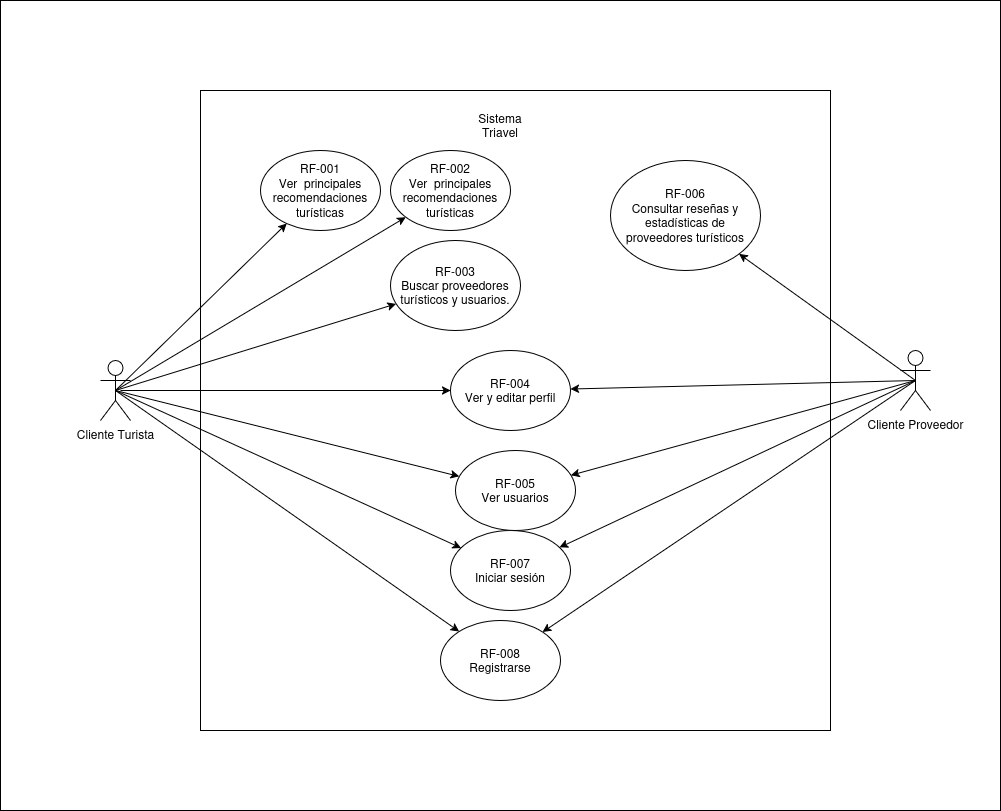
\includegraphics[width=0.9\textwidth]{Content/Images/CasosDeUso.png}
    \footnote{Nota. \textup{Fuente : Autores.}}
    \end{minipage}
    %------------------------------------------------------------------%


\textbf{Vistas principales del prototipo}
En función de los requisitos funcionales, no funcionales y los casos de uso definidos, a continuación se presentan en las figuras \ref{prot1}, \ref{prot2}, \ref{prot3}, \ref{prot4}, \ref{prot5}, \ref{prot6}, \ref{prot7}, \ref{prot8}, \ref{prot9}, \ref{prot10}, \ref{prot11}, \ref{prot12} las principales vistas que conforman el núcleo del plan de negocio. Todas las imágenes mostradas en este prototipo fueron diseñadas y desarrolladas exclusivamente para este proyecto.

    \vspace{2mm}
    \begin{minipage}{0.9\textwidth}
    \centering
    \captionof{figure}[{Vista principal parte I}]{Vista principal parte I}
    \label{prot1}
    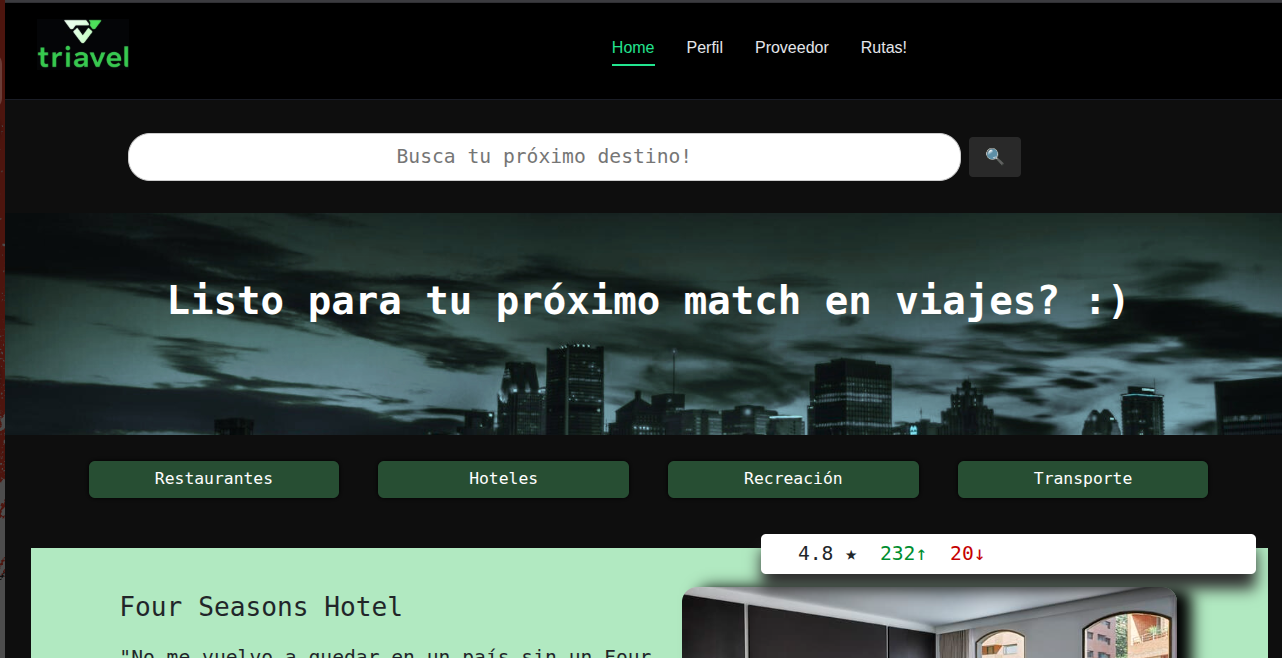
\includegraphics[width=0.9\textwidth]{Content/Images/VistaGeneral1.png}
    \footnote{Nota. \textup{Fuente: Autores}}
    \end{minipage}

    \vspace{2mm}
    \begin{minipage}{0.9\textwidth}
    \centering
    \captionof{figure}[{Vista principal parte II}]{Vista principal parte II}
    \label{prot2}
    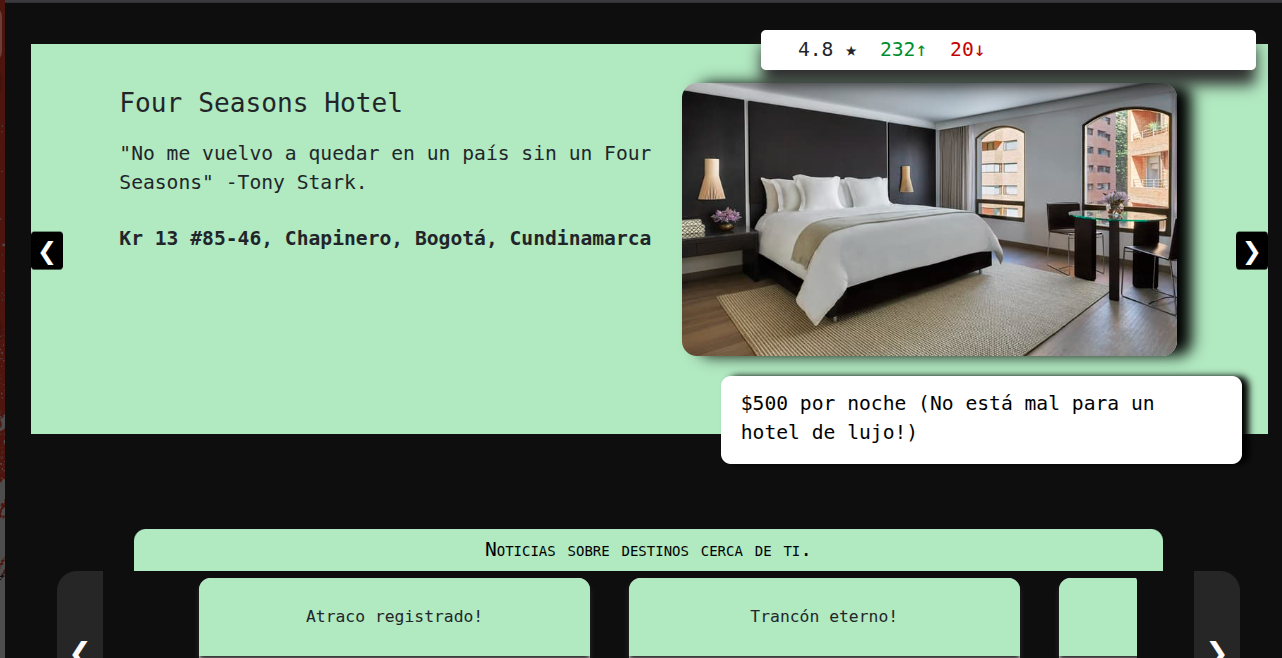
\includegraphics[width=0.9\textwidth]{Content/Images/VistaGeneral2.png}
    \footnote{Nota. \textup{Fuente: Autores}}
    \end{minipage}

    \vspace{2mm}
    \begin{minipage}{0.9\textwidth}
    \centering
    \captionof{figure}[{Vista principal parte III}]{Vista principal parte III}
    \label{prot3}
    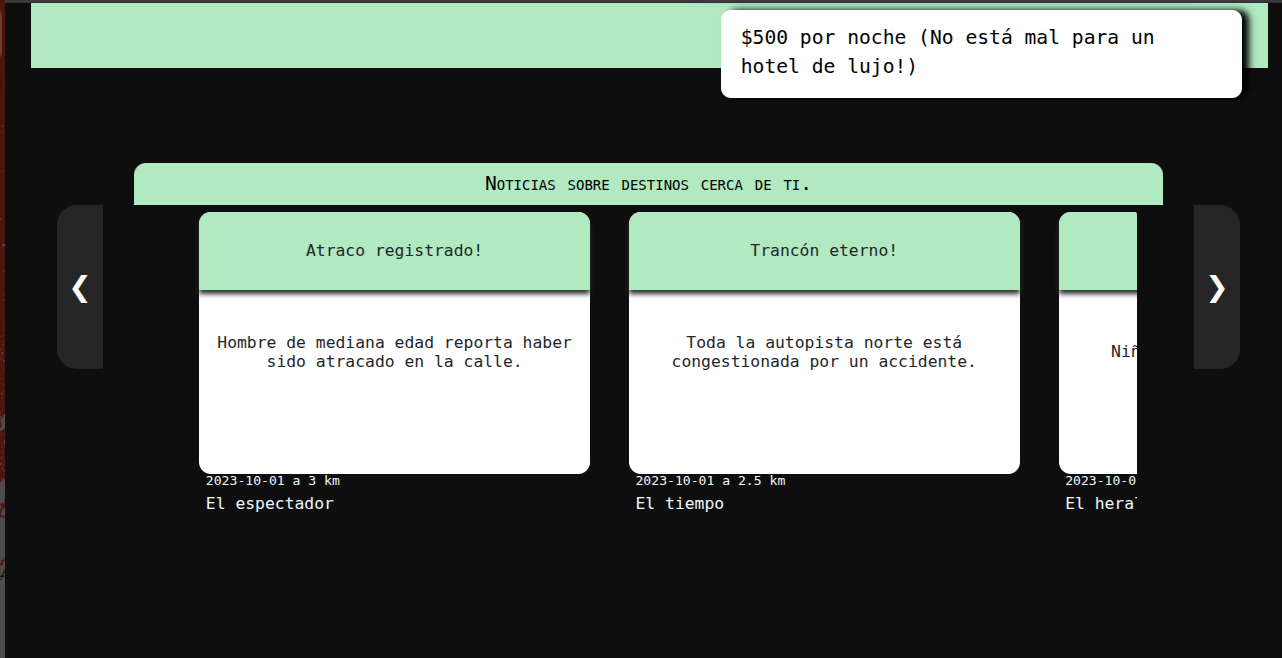
\includegraphics[width=0.9\textwidth]{Content/Images/VistaGeneral3.png}
    \footnote{Nota. \textup{Fuente: Autores}}
    \end{minipage}

    \vspace{2mm}
    \begin{minipage}{0.9\textwidth}
    \centering
    \captionof{figure}[{Tu Perfil}]{Tu Perfil}
    \label{prot4}
    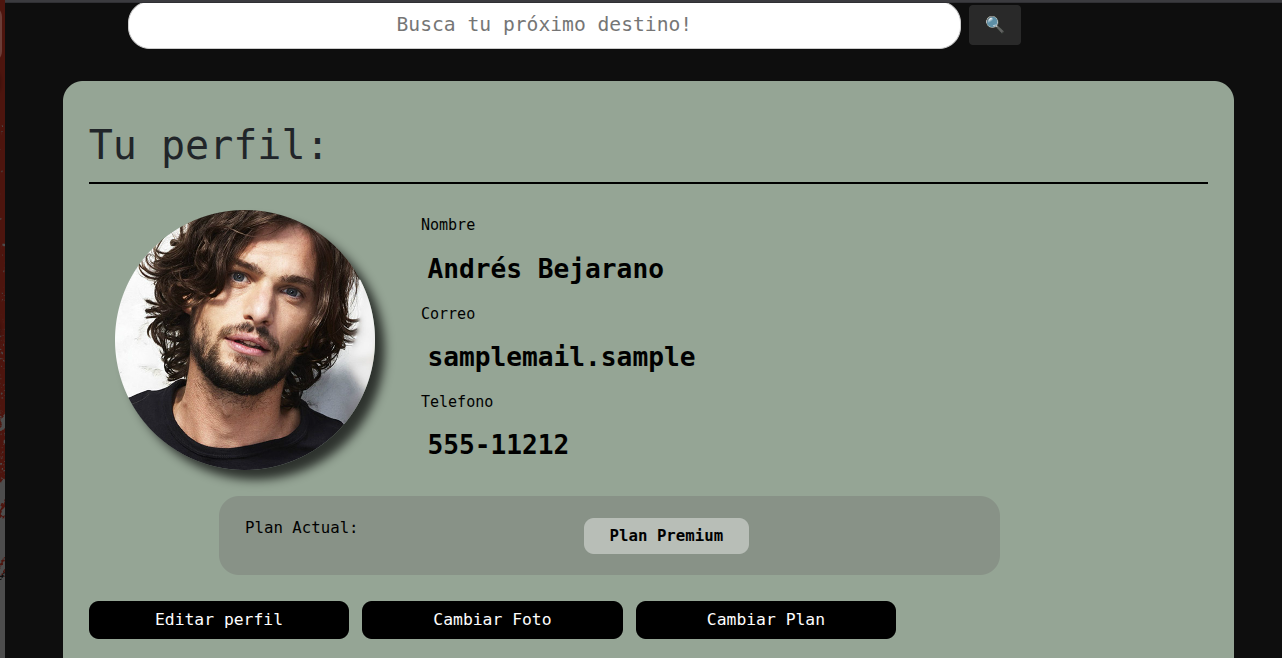
\includegraphics[width=0.9\textwidth]{Content/Images/TuPerfil.png}
    \footnote{Nota. \textup{Fuente: Autores}}
    \end{minipage}

     \vspace{2mm}
    \begin{minipage}{0.9\textwidth}
    \centering
    \captionof{figure}[{Vista de proveedor Parte I}]{Vista de proveedor Parte I}
    \label{prot5}
    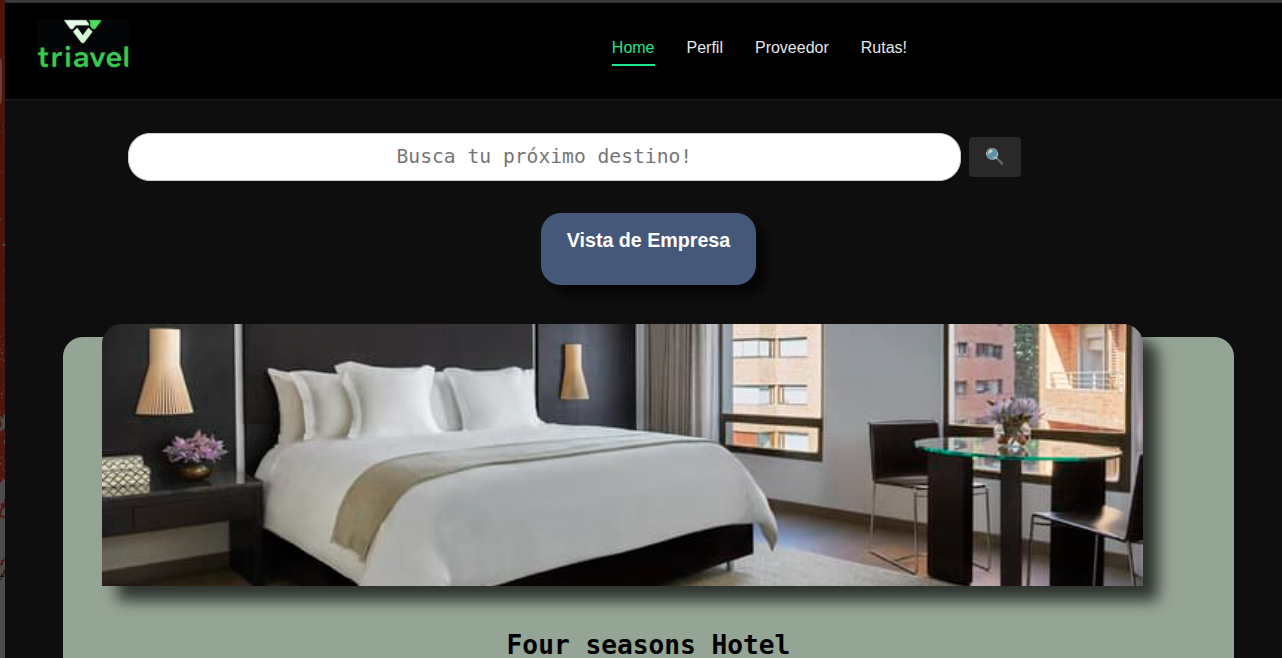
\includegraphics[width=0.9\textwidth]{Content/Images/VistaProveedor1.png}
    \footnote{Nota. \textup{Fuente: Autores}}
    \end{minipage}

     \vspace{2mm}
    \begin{minipage}{0.9\textwidth}
    \centering
    \captionof{figure}[{Vista de proveedor Parte II}]{Vista de proveedor Parte II}
    \label{prot6}
    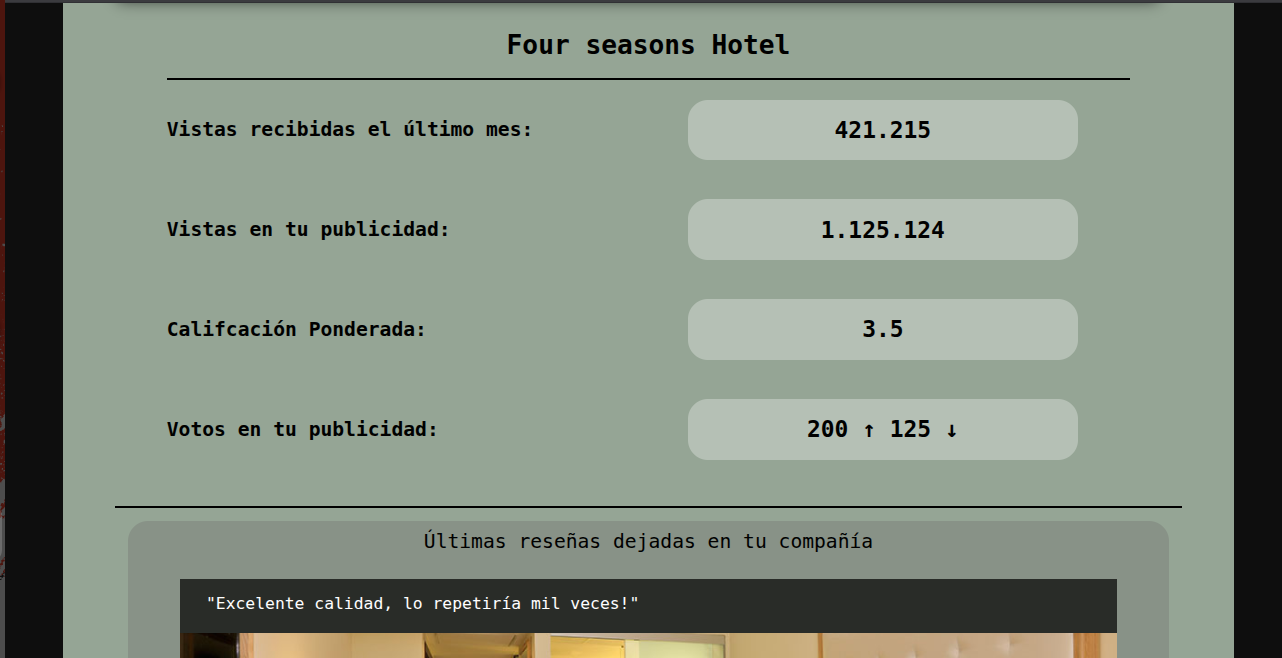
\includegraphics[width=0.9\textwidth]{Content/Images/VistaProveedor2.png}
    \footnote{Nota. \textup{Fuente: Autores}}
    \end{minipage}

     \vspace{2mm}
    \begin{minipage}{0.9\textwidth}
    \centering
    \captionof{figure}[{Vista de proveedor Parte III}]{Vista de proveedor Parte III}
    \label{prot7}
    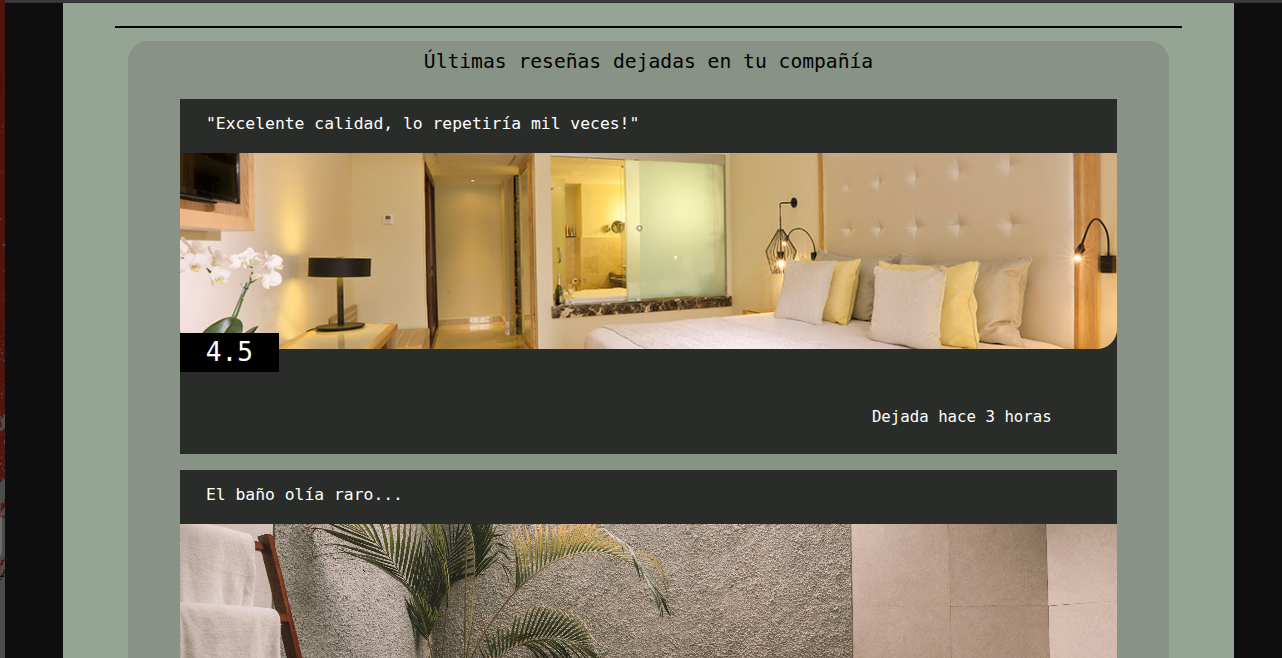
\includegraphics[width=0.9\textwidth]{Content/Images/VistaProveedor3.png}
    \footnote{Nota. \textup{Fuente: Autores}}
    \end{minipage}

     \vspace{2mm}
    \begin{minipage}{0.9\textwidth}
    \centering
    \captionof{figure}[{Ruta de viaje Parte I}]{Ruta de viaje Parte I}
    \label{prot8}
    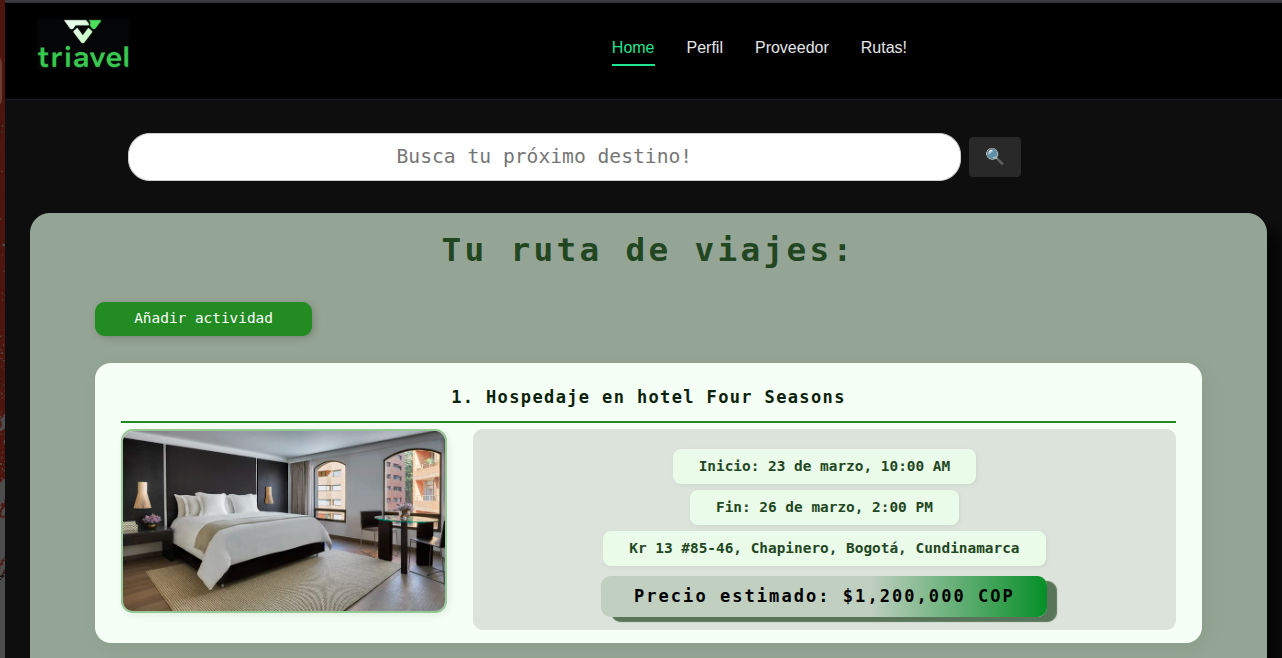
\includegraphics[width=0.9\textwidth]{Content/Images/RutaDeViaje1.png}
    \footnote{Nota. \textup{Fuente: Autores}}
    \end{minipage}

      \vspace{2mm}
    \begin{minipage}{0.9\textwidth}
    \centering
    \captionof{figure}[{Ruta de viaje Parte II}]{Ruta de viaje Parte II}
    \label{prot9}
    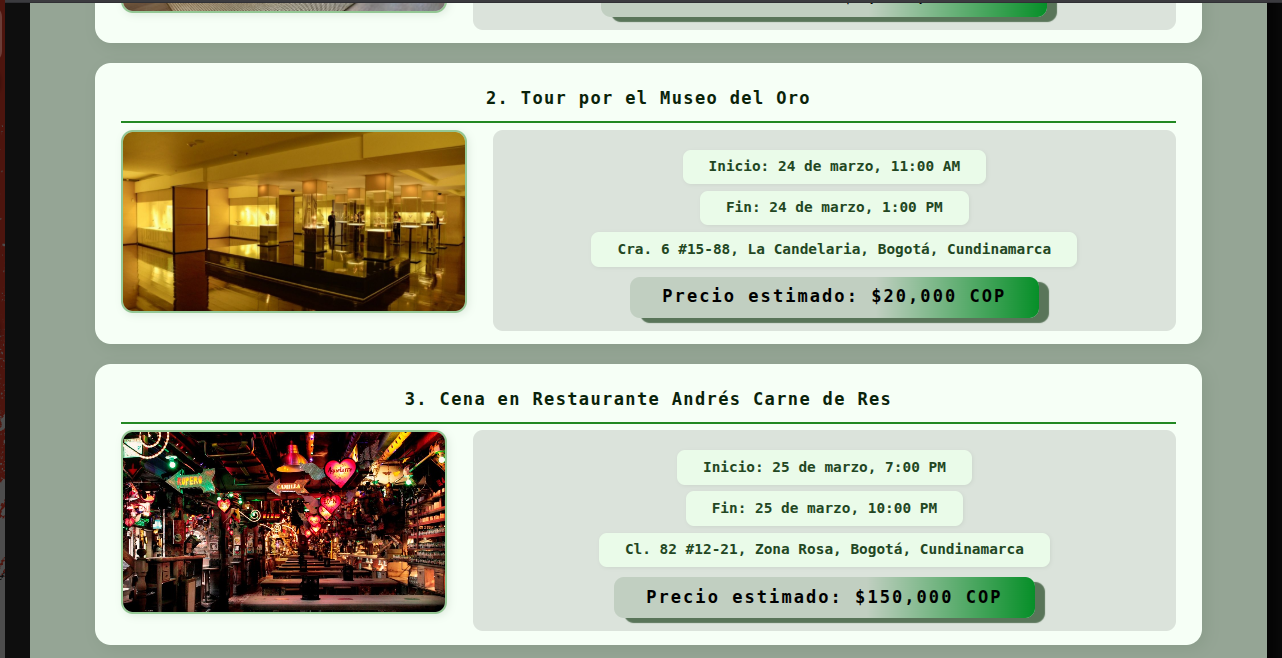
\includegraphics[width=0.9\textwidth]{Content/Images/RutaDeViaje2.png}
    \footnote{Nota. \textup{Fuente: Autores}}
    \end{minipage}

      \vspace{2mm}
    \begin{minipage}{0.9\textwidth}
    \centering
    \captionof{figure}[{Resultados de búsqueda}]{Resultados de búsqueda}
    \label{prot10}
    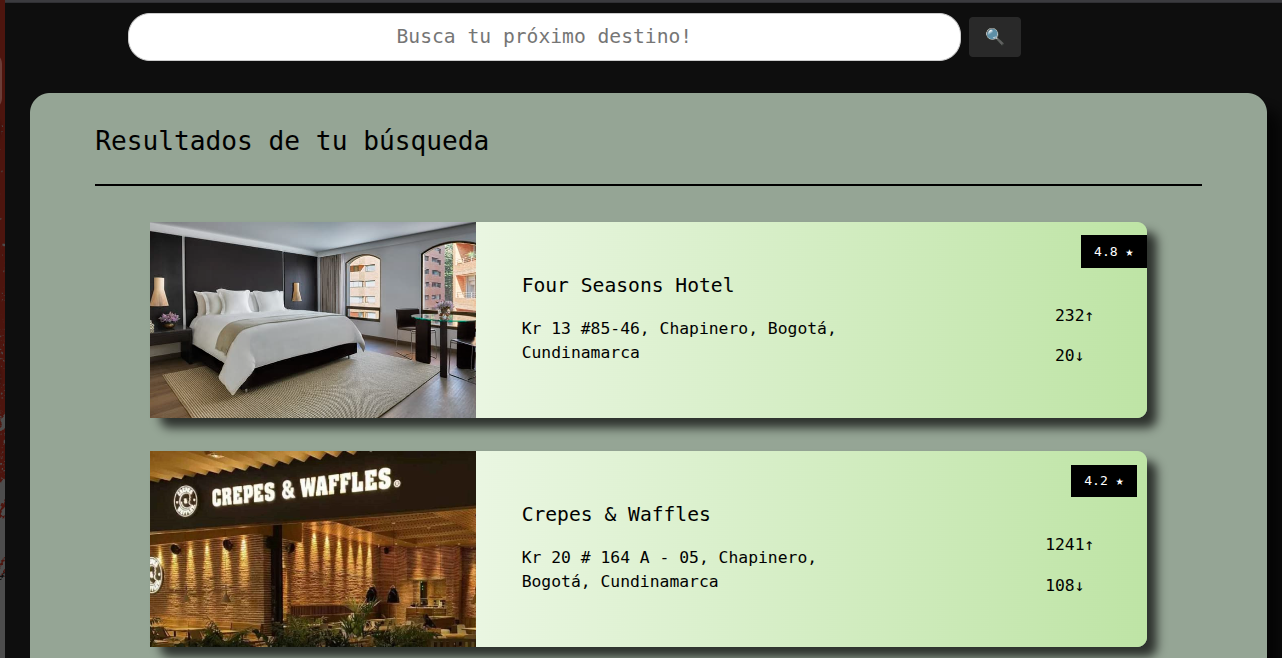
\includegraphics[width=0.9\textwidth]{Content/Images/ResultadosDeBusqueda.png}
    \footnote{Nota. \textup{Fuente: Autores}}
    \end{minipage}

       \vspace{2mm}
    \begin{minipage}{0.9\textwidth}
    \centering
    \captionof{figure}[{Vista de sitio}]{Vista de sitio}
    \label{prot11}
    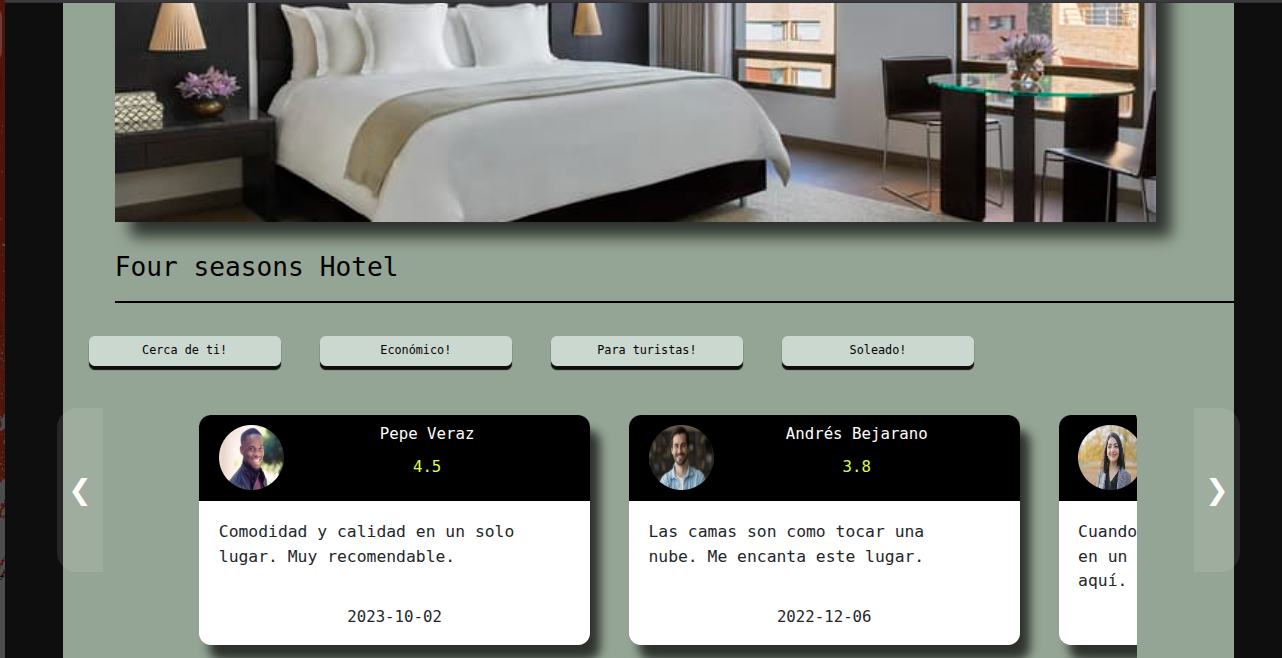
\includegraphics[width=0.9\textwidth]{Content/Images/VistaDeSitio.png}
    \footnote{Nota. \textup{Fuente: Autores}}
    \end{minipage}

      \vspace{2mm}
    \begin{minipage}{0.9\textwidth}
    \centering
    \captionof{figure}[{Perfil de usuario}]{Perfil de usuario}
    \label{prot12}
    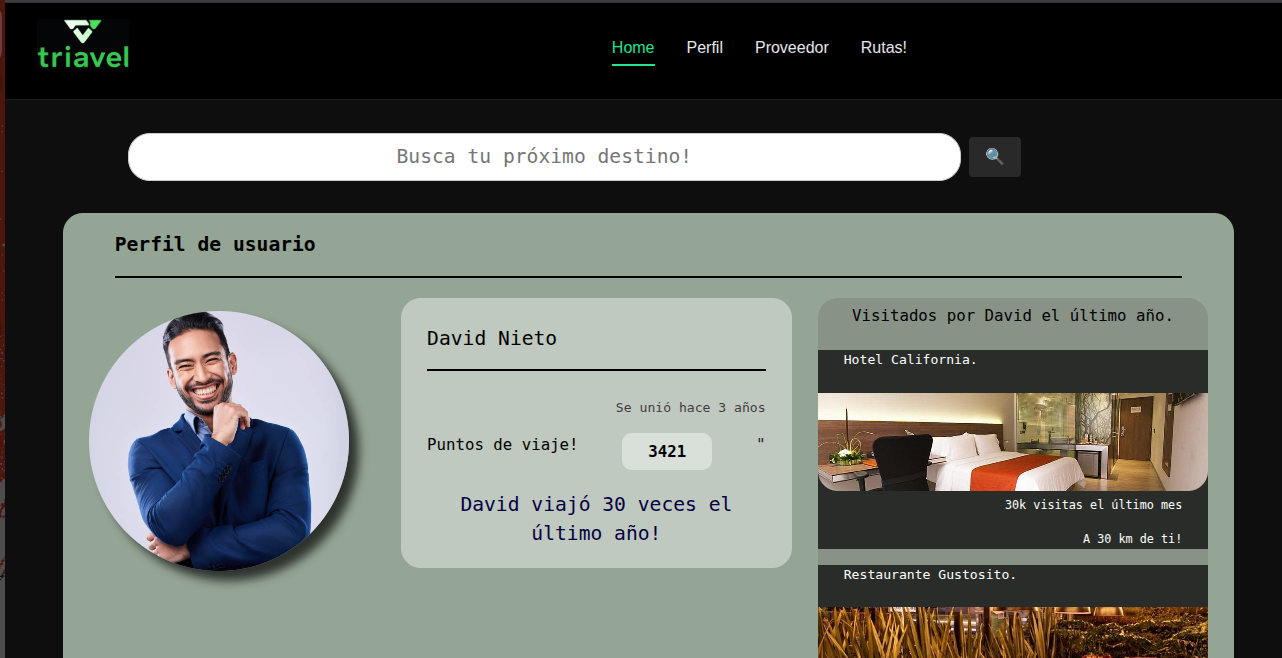
\includegraphics[width=0.9\textwidth]{Content/Images/UserProfile.png}
    \footnote{Nota. \textup{Fuente: Autores}}
    \end{minipage}


\subsection{Estudio legal}
El estudio legal es un análisis exhaustivo de la situación jurídica de una empresa, que busca identificar y evaluar los aspectos legales que pueden afectar su funcionamiento y desarrollo. Este estudio es fundamental para garantizar el cumplimiento normativo y la protección de los derechos e intereses de la empresa, así como para prevenir riesgos legales y financieros.

\subsection*{Tipo de sociedad}
Triavel se constituirá como una Sociedad por Acciones Simplificada (SAS) bajo la Ley 1258 de 2008, al igual que el 54\% de las empresas en Colombia, para aprovechar sus beneficios tributarios, flexibilidad operativa y costos reducidos. Esta estructura permite agilidad en trámites (constitución en 48 horas), no exige revisor fiscal en etapas iniciales y ofrece responsabilidad limitada para los socios, protegiendo su patrimonio personal. Además, facilita la atracción de inversionistas mediante acciones flexibles y adapta sus estatutos a las necesidades del negocio, priorizando escalabilidad internacional y eficiencia administrativa, clave para una startup tecnológica en el sector de seguridad para nómadas digitales.

\textbf{Especificaciones generales}
\newline

La empresa será construida bajo las siguientes pautas:

\begin{itemize}
    \item \textbf{Socios : } Andrés Felipe Bejarano Barón con Cédula de Ciudadanía No ----- y Jeferson David Nieto Gaona con Cédula de Ciudadanía No 1001272402 
    \item \textbf{Nombre de la empresa :} Traivel S.A.S
    \item \textbf{Duración :} Tiempo indefinido.
    \item \textbf{Objeto social :} Empresa cuyo objeto se encuentra en el desarrollo e innovación de herramientas tecnológicas.
    \item \textbf{Responsabilidad sobre los aportes :} 50/50 entre socios.
    \item \textbf{Representante legal: } Andrés Felipe Bejarano Barón
\end{itemize}

\subsection*{Obligaciones legales}
Las obligaciones legales establecidas por la Ley 1258 de 2008 para las SAS incluyen:
\begin{enumerate}
    \item Registro ante la camara de comercio.
    \item Inscripción en el Registro Único Tributario (RUT) ante la DIAN.
    \item Obtención del NIT (Número de Identificación Tributaria).
    \item Registro de libros contables y actas.
    \item Inscripción de los socios y accionistas en el libro de registro de acciones.
    \item Afiliación a la seguridad social de los empleados.
    \item Presentación de declaraciones tributarias (IVA, renta, retención en la fuente).
    \item Cumplimiento de las obligaciones laborales y de seguridad social.
\end{enumerate}

\subsection*{Proceso para disolución de la empresa}
\begin{enumerate}

    \item La disolución de la empresa puede ser voluntaria o forzosa, y debe ser aprobada por la asamblea de accionistas.
    \item Se debe elaborar un acta de disolución y registrarla en la cámara de comercio.
    \item Nombrar un liquidador que se encargue de liquidar los activos y pasivos de la empresa, realizando el inventario correspondiente.
    \item Publicar un aviso de disolución en un medio de comunicación local.
    \item Liquidar los activos y pasivos de la empresa, y distribuir el remanente entre los socios,al pagar las obligaciones se debe priorizar los salarios y las prestaciones sociales, seguido de los impuestos correspondientes a la DIAN.
    \item Presentar la declaración final de renta ante la DIAN.
    \item \item Realizar el acta de liquidación con detalle en activos vendidos, pasivos pagados y remanente distribuido entre socios.
    \item Registrar la liquidación en la cámara de comercio,cancelar la matrícula mercantil y liquidar cuentas bancarias.
    \item Cancelar el registro de los libros contables y actas.
\end{enumerate}

\subsection*{Propiedad intelectual}
La propiedad intelectual es un conjunto de derechos que protegen las creaciones de la mente, como invenciones, obras literarias y artísticas, diseños industriales y marcas. En el caso de Triavel, la propiedad intelectual es fundamental para proteger su software y tecnología desarrollada. Para ello, se recomienda registrar el software ante la Dirección Nacional de Derechos de Autor y considerar la posibilidad de patentar invenciones o diseños industriales relacionados con su producto.Es importante establecer acuerdos de confidencialidad con empleados y colaboradores para proteger información sensible y secretos comerciales,además se debe incluir cláusulas en los estatutos de la SAS que reconozcan el software como un activo intangible de la sociedad, asegurando su titularidad y control legal .


\subsection{Estudio Ambiental}

El desarrollo de software en Colombia está regulado por la Ley 23 de 1982 (derechos de autor), Ley 603 del 2000 (protección y comercialización de software) y la Ley 1581 de 2012 (protección de datos personales). El proyecto cumplirá estas normativas, garantizando la protección de datos y la correcta declaración del software.

\subsection*{Impactos ambientales}

Triavel reconoce los impactos ambientales de sus operaciones tecnológicas y se compromete a gestionarlos responsablemente durante todo el ciclo de vida del producto, planificando el uso de recursos tecnológicos e infraestructura digital.

\subsection*{Políticas ambientales}

Triavel cumple el Decreto 1076 de 2015 (SINA) y la Ley 1715 de 2014, adoptando acciones como:
\begin{itemize}
    \item Uso de energía renovable en proveedores cloud (Ley 1715).
    \item Gestión de residuos electrónicos según el Decreto 284 de 2018 (RAEE).
    \item Medición y compensación de huella de carbono (Resolución 40807 de 2018) mediante apoyo a proyectos de conservación.
\end{itemize}
La app promueve rutas seguras y eco-amigables, fomentando el turismo responsable.


%-------------ANALISIS FINANCIERO---------------------%
\section{Análisis financiero}

\import{./}{Content/10.AnalisisFinanciero/InversionInicial}

\import{./}{Content/10.AnalisisFinanciero/Establecimiento}

\import{./}{Content/10.AnalisisFinanciero/IngresosEgresos}

\import{./}{Content/10.AnalisisFinanciero/ProyeccionDeVentas}

\import{./}{Content/10.AnalisisFinanciero/AmortizacionDepreciacion}

\import{./}{Content/10.AnalisisFinanciero/BalanceGeneral}

\import{./}{Content/10.AnalisisFinanciero/EstadoDeResultados}

\import{./}{Content/10.AnalisisFinanciero/FlujoDeCaja}

\import{./}{Content/10.AnalisisFinanciero/FlujoDeEfectivos}



%-------------ANALISIS INTERNO---------------------%
\section{Análisis interno y externo}



\subsection{Matriz PEYEA}
Esta matriz permite definir si una estrategia activa, conservadora, defensiva o competitiva es la más adecuada para una organización dada. Los ejes de la matriz representan dos dimensiones internas (fuerza financiera y ventaja competitiva) y dos externas (fuerza de la industria y estabilidad del ambiente). Se seleccionan variables para cada una de las dimensiones; se les adjudica una calificación con un valor numérico de 1 a 6, o –1 a –6, donde 1 representa la mejor calificación en valor absoluto; se calcula la calificación promedio de cada dimensión; se anotan las calificaciones promedio de cada dimensión en el eje correspondiente; se suman las dos calificaciones del eje X para obtener una primera coordenada, y se repite para el eje de las Y; por último, se traza un vector del origen al punto encontrado para ubicar en un cuadrante el perfil que la empresa debiera buscar para orientar su estrategia.\cite{DOFA}

la definicion del acronimo PEYEA es la siguiente:
\begin{itemize}
    \item \textbf{P - Posición Estratégica:} Es la situación actual de la empresa en el mercado.
    \item \textbf{E - Evaluación:} Es el análisis de la posición estratégica actual.
    \item \textbf{Y - Yuxtaposición:} Es la comparacion de la posición estratégica con las condiciones del mercado y la competencia.
    \item \textbf{E - Estrategia:} Teniendo en cuenta la evaluación y analisis se plantea una estrategia.
    \item \textbf{A - Acción:} Son las acciones que se deben realizar para llevara cabo la estrategia planteada.
\end{itemize}

\subsection{Pasos para elaborar una matriz PEYEA}

\begin{enumerate}
    \item \textbf{Seleccionar Variables:} Elegir una serie de variables que representen las cuatro dimensiones de la matriz (Fuerzas Financieras, Ventaja Competitiva, Estabilidad del Ambiente y Fuerza de la Industria). Resaltando la importancia de estas variables para la organización y el mercado.
    \item \textbf{Asignar Valores Numéricos:} Asignar un valor numérico a cada variable. Para las Fuerzas Financieras(FF) y Fuerza de la Industria(FI), utilizar una escala de +1 (peor) a +6 (mejor). Para Ventaja Competitiva(VC) y Estabilidad del Ambiente(EA), utilizar una escala de -1 (mejor) a -6 (peor).
    \item \textbf{Calcular la Calificación Promedio:} se suman los valores resultantes de las variables de cada dimensión y se divide el total por la cantidad de variables para obtener la media.
    \item \textbf{Anotar en la Matriz:} Ubicar los valores resultados en el calculo anterior de cada factor en el eje correspondiente de la matriz.
    \item \textbf{Sumar los Valores de los Ejes:} Sumar los valores medios de las Fuerzas Financieras y Ventaja Competitiva para el eje vertical, y Estabilidad del Ambiente y Fuerza de la Industria para el eje horizontal.
    \item \textbf{Determinar la Posición Estratégica:} Dependiendo de la intersección de los valores en la matriz se adopatará la estrategia recomendable ya sea agresiva, conservadora, defensiva o competitiva.
    \item \textbf{Trazar un Vector Direccional:} Desde el origen de la matriz hasta el punto de intersección,se debe trazar un vector.Dando guia del tipo de estrategia más adecuada para la organización.
\end{enumerate}

Comprendiendo los conceptos y pasos descritos anteriormente, se procede a elaborar la matriz PEYEA para la empresa en cuestión. Esta matriz permitirá identificar las estrategias más adecuadas para mejorar el desempeño de la compañía en el mercado y determinar si estas son agresivas, conservadoras, defensivas o competitivas.

\vspace{2mm}
\begin{minipage}{0.9\textwidth}
\centering
\captionof{table}[{Matriz PEYEA.}]{ Matriz PEYEA }
\label{peyea}
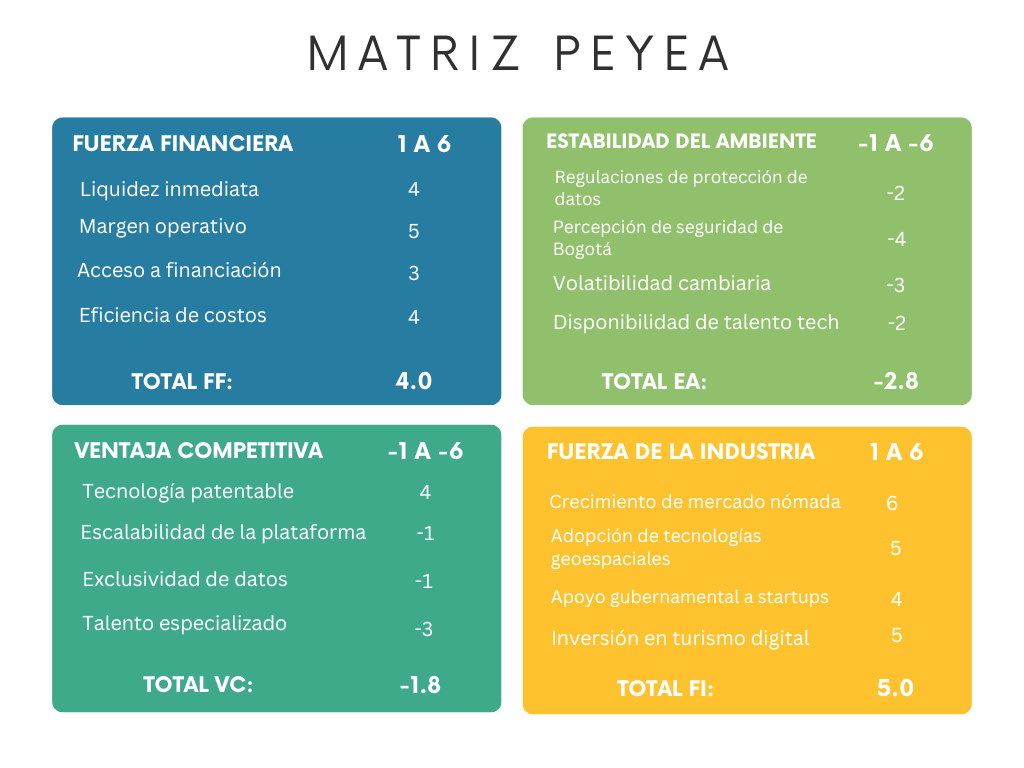
\includegraphics[scale=0.5]{Content/Images/Matriz PEYEA.png}
%\fnote{Nota. \textup{Fuente : Autores.}}
\end{minipage}

Para determinar el valor de X, se sumaron los valores de Ventaja Competitiva (VC) y Fuerza de la Industria (FI).Como se muestra a continuación:
\begin{align*}
X &= VC + FI \\
X &= -1.8+5 \\
X &= 3.2
\end{align*}

El valor de Y se obtuvo sumando Fuerza Financiera (FF) y Estabilidad del Ambiente (EA).Como se muestra a continuación:
\begin{align*}
Y &= FF + EA \\
Y &= 4.0-2.8 \\
Y &= 1.2
\end{align*}

Dichos valores se representan gráficamente en la siguiente imagen:

\vspace{2mm}
\begin{minipage}{0.9\textwidth}
\centering
\captionof{figure}[{Representación gráfica Matriz PEYEA.}]{ Representación gráfica Matriz PEYEA }
\label{peyeagrafico}
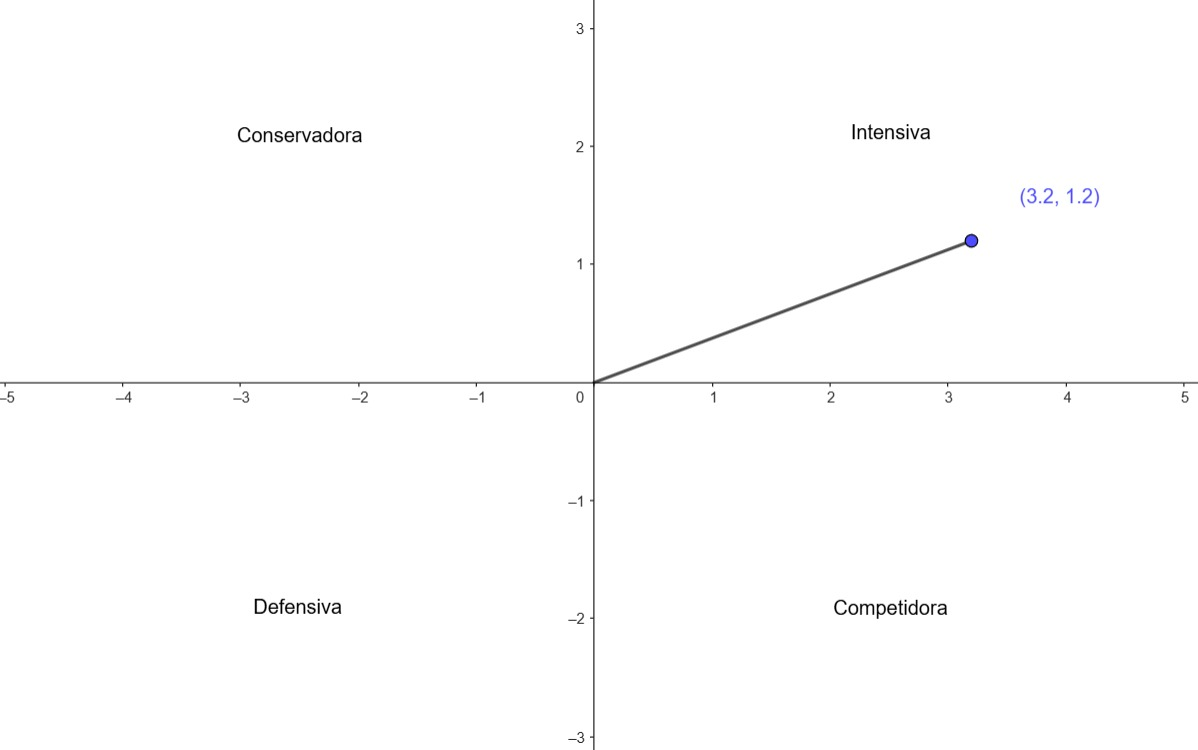
\includegraphics[width=1\textwidth]{Content/Images/PEYEA.jpeg}
%\fnote{Nota. \textup{Fuente : Autores.}}
\end{minipage}

Como conclusión, se obtiene que el proyecto se encuentra en el primer cuadrante de la matriz PEYEA, indicando que se debe seguir una estrategia intensiva. Indicando que las fortalezas internas son un pilar importante para maximizar las oportunidades externas, explotando las ventajas competitivas y la fuerza financiera del proyecto. Permitiendo maxificar las fortalezas y oportunidades, minimizando las debilidades y amenazas,garantizando así un crecimiento sostenido y una posición competitiva sólida en el mercado para el proyecto.
%------------------------------------------------------------------

\color{black}
\subsection{Matriz DOFA}
Estas siglas provienen del acrónimo en inglés SWOT (strenghts, weaknesses, opportunities, threats); en español, aluden a fortalezas, oportunidades, debilidades y amenazas. El análisis FODA consiste en realizar una evaluación de los factores fuertes y débiles que, en su conjunto, diagnostican la situación interna de una organización, así como su evaluación externa, es decir, las oportunidades y amenazas. También es una herramienta que puede considerarse sencilla y que permite obtener una perspectiva general de la situación estratégica de una organización determinada. Thompson y Strikland (1998) establecen que el análisis FODA estima el efecto que una estrategia tiene para lograr un equilibrio o ajuste entre la capacidad interna de la organización y su situación externa, esto es, las oportunidades y amenazas. \cite{Dofa}

En la siguiente figura se ilustran los elementos que componen el análisis FODA y como identificarlos:

\vspace{2mm}
\begin{minipage}{0.9\textwidth}
\centering
\captionof{figure}[{Aspectos Matriz DOFA.}]{ Aspectos Matriz DOFA }
\label{dofa}
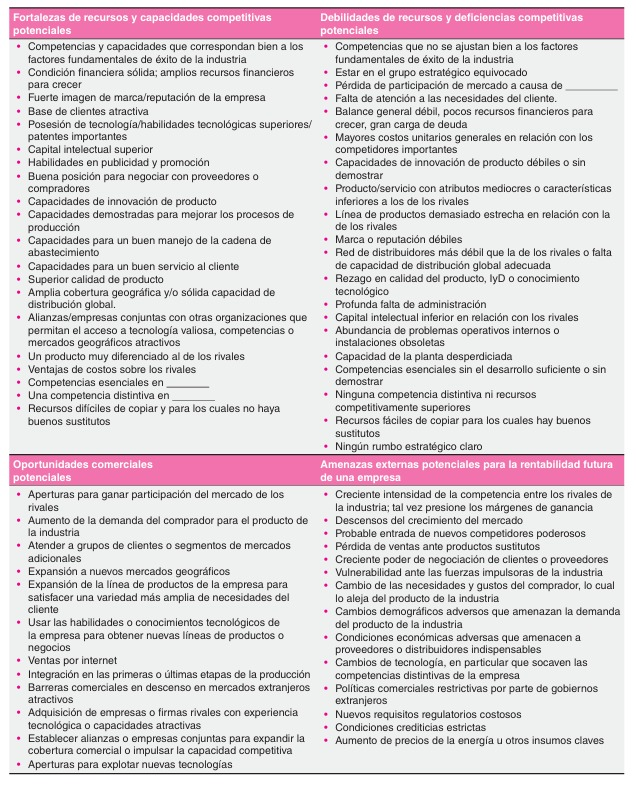
\includegraphics[width=1.2\textwidth]{Content/Images/dofa-ejemplo.jpeg}
\footnote{Nota. \textup{Fuente :Administracion estrategica
\cite{administracion-estrategica}}}
\end{minipage}

Agrupando los elementos del análisis FODA, se pueden identificar cuatro tipos de estrategias:
\begin{itemize}
     \item \textbf{FO(Fortalezas-Oportunidades):}Estas estrategias permiten a la organización crecer y desarrollarse aprovechando al máximo sus capacidades internas y las oportunidades que ofrece el entorno. Por ejemplo, una empresa con una sólida reputación y recursos tecnológicos avanzados puede expandirse a nuevos mercados emergentes o lanzar productos innovadores, capitalizando tanto sus fortalezas como las oportunidades detectadas.
    \item \textbf{DO (Debilidades-Oportunidades):} Estrategias que buscan mejorar las debilidades internas aprovechando las oportunidades externas disponibles. Estas estrategias pueden implicar la inversión en capacitación del personal, la mejora de procesos internos o la adopción de nuevas tecnologías para optimizar el rendimiento y la competitividad de la organización.
    \item \textbf{FA (Fortalezas-Amenazas):} Estrategias que utilizan las fortalezas internas para enfrentar y mitigar las amenazas externas que enfrenta la organización. Por ejemplo, una empresa con una sólida red de distribución puede utilizarla para contrarrestar la competencia agresiva o adaptarse a cambios en las regulaciones del mercado, asegurando así su posición en el sector.
    \item \textbf{DA (Debilidades-Amenazas):} Estrategias defensivas que buscan minimizar las debilidades internas y evitar o reducir el impacto de las amenazas externas en la organización. Estas estrategias pueden incluir la reestructuración de procesos, la mejora de la eficiencia operativa o la diversificación de productos y servicios para reducir la dependencia de un mercado específico.
\end{itemize}

\begin{minipage}{0.9\textwidth}
\centering
\captionof{table}[{ Matriz DOFA.}]{  Matriz DOFA }
\label{dofa}
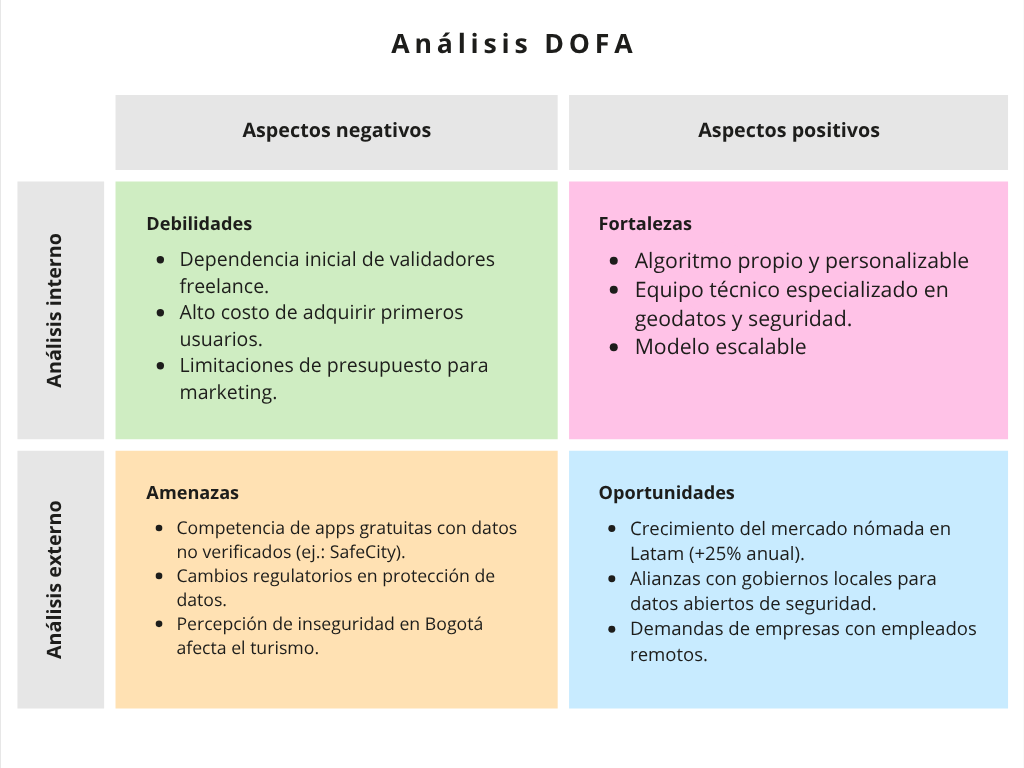
\includegraphics[width=1.2\textwidth]{Content/Images/Matriz-dofa-proyecto.png}
\footnote{Nota. \textup{Fuente : Autores.}}
\end{minipage}




\subsection{Análisis DOFA}
\begin{minipage}{0.9\textwidth}
\centering
\captionof{table}[{ Analisis DOFA.}]{  Analisis DOFA }
\label{dofa}
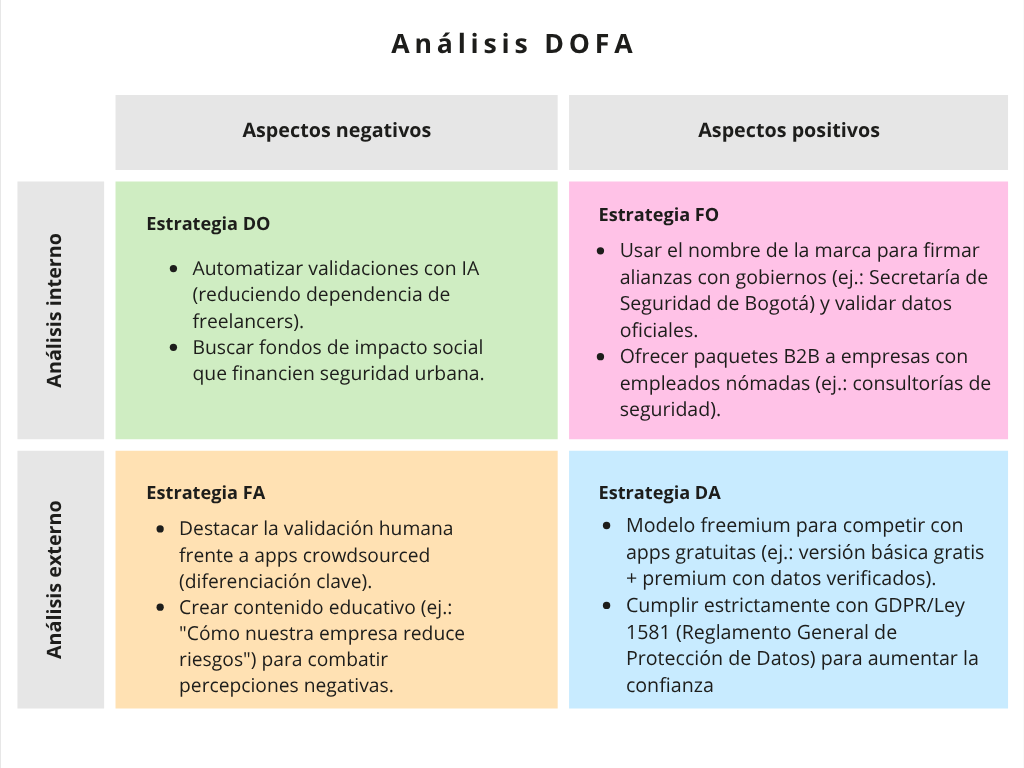
\includegraphics[scale=0.4]{Content/Images/analisis-dofa.png}
\footnote{Nota. \textup{Fuente : Autores.}}
\end{minipage}

%-------------ANALISIS DE RIESGO---------------------%
\section{Análisis de riesgo}
De acuerdo con el Artículo 1 de la Ley 1523 de 2012, la gestión del riesgo de desastres es un proceso social orientado a la formulación, ejecución, seguimiento y evaluación de políticas, estrategias, planes, programas, regulaciones, instrumentos, medidas y acciones permanentes para el conocimiento y la reducción del riesgo y para el manejo de desastres, con el propósito explícito de contribuir a la seguridad, el bienestar, la calidad de vida de las personas y al desarrollo sostenible. 

El análisis de riesgo es un proceso que permite identificar, evaluar y priorizar los riesgos asociados a una organización o proyecto. Este proceso es esencial para la toma de decisiones informadas y para la implementación de medidas que minimicen los impactos negativos de los riesgos identificados.

\color{red}

\subsection{Factores limitantes y obstáculos}

Los proyectos empresariales suelen enfrentar una serie de desafíos y obstáculos que forman parte integral de su evolución. Estos retos pueden surgir de la interacción entre el equipo humano, los procesos operativos y las soluciones tecnológicas implementadas. A lo largo del tiempo, esta realidad ha impactado a empresas de todo tipo, manifestándose de diversas maneras y teniendo causas múltiples. La frecuente aparición de pérdidas significativas en el ámbito empresarial indica una falta de comprensión sobre estos factores clave, así como la ausencia de métodos efectivos para su control y gestión. Por ello, es fundamental identificar y gestionar eficientemente estos elementos limitantes para mitigar su impacto negativo y asegurar el crecimiento y éxito de los proyectos empresariales.\cite{AdministrarProyectos}.


\color{red}
\subsection{Factores claves de éxito}

Los Factores Críticos de Éxito (FCE) son aquellas cualidades, recursos o capacidades altamente valorados por un segmento específico de clientes, y que una organización debe dominar para sobresalir frente a la competencia. Estos FCE constituyen los cimientos esenciales que soportan el éxito de una empresa en el mercado \cite{Asana}. Algunos de estos factores incluyen:

\begin{itemize}
    \item Estrategia de precios
    \item Estrategias de publicidad y marketing.
    \item Calidad del producto o servicio ofrecido. 
    \item Fidelización y satisfacción del cliente.
    \item Conocimiento profundo del mercado y sus necesidades.
    \item Planificación estratégica sólida. 
    \item Innovación continua en productos, servicios o procesos. 
    \item Capacidad de escalabilidad del producto o servicio para adaptarse al crecimiento y demanda del mercado. 
\end{itemize}


\color{red}
\subsection{Riesgos legales}

El riesgo legal se refiere a la posibilidad de incumplir leyes, normativas y regulaciones emitidas por los gobiernos de cada país o por otras entidades. Este riesgo puede surgir tanto por desconocimiento de una ley o norma específica como por su omisión deliberada. Asimismo, el riesgo legal también abarca el incumplimiento de contratos y acuerdos comerciales con terceros \cite{pira}.

\textbf{Riesgo:} Protección de la empresa ineficiente.

\textbf{Mitigación:} Se establecerán políticas internas para garantizar un manejo correcto de la propiedad intelectual, marcas registradas, bases de datos y otros activos de la empresa. Además, se contará con un equipo legal especializado para asegurar la adecuada protección de los derechos y activos de la organización.

\textbf{Riesgo:} Reclamos y acciones legales.

\textbf{Mitigación:} Se contratarán servicios de asesoría legal especializada para gestionar cualquier reclamación o acción legal que pueda surgir. Estos profesionales representarán a la empresa en procesos legales, investigaciones y procedimientos administrativos, contribuyendo a minimizar el riesgo de multas y sanciones.

\textbf{Riesgo:} Uso de software sin licencia.


\textbf{Mitigación:} Se establecerán políticas claras de licenciamiento de software que regulen el uso adecuado de programas, tanto libres como de pago. Un equipo especializado se encargará de supervisar el cumplimiento de estas políticas y garantizar que todos los programas utilizados cuenten con la licencia correspondiente.

\textbf{Riesgo:} Incumplimiento de contratos.


\textbf{Mitigación:} Se buscará la asesoría de profesionales legales para redactar y ejecutar contratos, asegurando que estos reflejen de manera clara y precisa los términos y condiciones de los acuerdos comerciales. Además, se establecerán procesos internos para garantizar que la empresa cumpla con sus compromisos contractuales.

\textbf{Riesgo:} Disputas contractuales con proveedores o clientes.


\textbf{Mitigación:} Se establecerán cláusulas claras y detalladas en los contratos con proveedores y clientes, definiendo los derechos y responsabilidades de ambas partes, así como los procedimientos para la resolución de disputas. Además, se designará un punto de contacto específico para gestionar las comunicaciones y resolver cualquier inconveniente de manera oportuna y efectiva.

\textbf{Riesgo:} Publicidad Engañosa.


\textbf{Mitigación:} Para prevenir la publicidad engañosa o falsa, se garantizará que toda la comunicación publicitaria sea veraz y precisa. No se realizarán promesas que no puedan cumplirse ni se empleará información falsa o engañosa para atraer a los usuarios. Además, se implementará un sistema de revisión y aprobación de la publicidad para asegurar que cumpla con los estándares establecidos.

\section{Riesgos operacionales}
El Comité de Basilea define al riesgo operacional como al riesgo de pérdidas resultantes de la falta de adecuación o fallas en los procesos internos, de la actuación del personal o de los sistemas o bien aquellas que sean producto de eventos externos.

\textbf{Riesgo:}Interrupciones en APIs de proveedores
\textbf{Contra medida:} Se implementará un sistema de caché inteligente para respuestas de APIs críticas y se establecerán conexiones redundantes con múltiples proveedores en cada categoría. Además, se desarrollará un módulo de "modo offline" que permita operaciones básicas cuando los servicios externos no estén disponibles, garantizando continuidad en la experiencia del usuario.

\textbf{Riesgo:} Inexactitud en información dinámica
\textbf{Contra medida:}Se implementará un sistema de verificación automatizada que cruce datos de múltiples fuentes en tiempo real y alertas de discrepancia. Además, se establecerá un protocolo de actualización horaria con proveedores y un equipo dedicado para corrección manual inmediata de datos críticos reportados por usuarios.

\textbf{Riesgo:}Sobrecarga en la plataforma
\textbf{Contra medida:} Se implementará un sistema de balanceo de carga avanzado que distribuya el tráfico de manera equitativa entre múltiples servidores. Además, se establecerán límites de uso por usuario y se implementarán mecanismos de escalabilidad automática para aumentar la capacidad durante picos de tráfico.

\textbf{Riesgo:}Vulneraciones en pagos en línea y datos sensibles de usuarios
\textbf{Contra medida:} Se integrarán soluciones de tokenización PCI-DSS para procesamiento de pagos y se implementará autenticación multifactor obligatoria para todas las cuentas con acceso a datos sensibles. Además, se realizarán auditorías de seguridad trimestrales por terceros especializados y cifrado de extremo a extremo para toda información financiera.
\textbf{Riesgo:}Contenido fraudulento o engañoso en reseñas y perfiles
\textbf{Contra medida:} Se implementará un sistema de verificación de identidad por dos pasos para creadores de contenido y algoritmos de detección de patrones fraudulentos. Además, se establecerá un equipo de moderación especializado y un sistema de reputación basado en interacciones validadas por la comunidad.

\textbf{Riesgo:}Fallos de integración de sistemas de partners
\textbf{Contra medida:} Se establecerán acuerdos de nivel de servicio (SLA) claros con todos los partners y se implementará un sistema de monitoreo continuo de integraciones. Además, se desarrollarán pruebas automatizadas para cada nueva integración y se establecerá un protocolo de respuesta rápida para resolver fallos críticos en menos de 24 horas.



%-------------ANALISIS IMPACTOS---------------------%
\section{Impactos}

\subsection{Impacto social}

A corto plazo, el proyecto mejorará la integración social de los nómadas digitales en Bogotá, mediante comunidades virtuales que faciliten conexiones auténticas con locales y otros nómadas. Se fomentará la participación en actividades comunitarias y eventos presenciales, promoviendo un sentido de pertenencia y colaboración, además de combatir el aislamiento social que a menudo enfrentan los nómadas digitales.

A mediano plazo, se fortalecerá el tejido social mediante la creación de redes de apoyo y colaboración entre nómadas digitales y residentes locales. Se implementarán programas de voluntariado y actividades conjuntas que fomenten el intercambio cultural y la inclusión social, contribuyendo a una comunidad más cohesionada y diversa.

A largo plazo, el proyecto aspira a transformarse en un puente global de cohesión social mediante la creación de "Hubs de convivencia sostenible" en diversas ciudades del mundo. Estos espacios integrarán a nómadas digitales en proyectos colaborativos que aborden desafíos sociales y ambientales locales, promoviendo un modelo de vida nómada que respete y enriquezca las comunidades anfitrionas. Se espera que esta iniciativa inspire a otras ciudades a adoptar enfoques similares, fomentando una cultura global de colaboración y sostenibilidad,sentando las bases para comunidades interculturales resilientes.




\subsection{Impacto Ambiental}
En un principio se propone un enfoque digital con la finalidad de disminuir la huella ambiental del proyecto, se fomentarán experiencias turisticas de bajo impacto como rutas caminables, cowokings verdes y alojamientos eco-certificados, que garanticen la seguridad y bienestar de los usuarios, al mismo tiempo que se promueve un estilo de vida saludable y activo.

Como parte del plan a mediano plazo se busca integrar criterios de sosstenibilidad en el algoritmo de recomendaciones, priorizando negocios locales que implementen prácticas sostenibles y responsables con el medio ambiente, además se lanzará un programa de compensación colaborativa donde cada reserva generará un aporte a proyectos de conservación ambiental.

Por ultimo se tiene como objetivo a largo plazo convertirse en un referente de turismo nomada sostenible, mediante un sistema de "Eco-score" que evalúe y promueva prácticas responsables entre los usuarios, incentivando un estilo de vida que respete y cuide el medio ambiente.


\subsection{Impacto económico}

En primer lugar, el proyecto generará empleo directo en áreas tecnológicas y de operaciones, mientras dinamiza economías locales atrayendo nómadas digitales a destinos emergentes como Bogotá. Esto incrementa el consumo en servicios como alojamientos, coworkings, restaurantes y transporte, beneficiando a la comunidad local.

A mediano plazo, se fortalecerán cadenas de valor turístico mediante alianzas con proveedores locales para ofertas integradas y experiencias auténticas. Se lanzarán programas de formación y capacitación para emprendedores locales, fomentando el desarrollo de habilidades en el sector turístico y tecnológico.

Manteniendo el enfoque a largo plazo, la plataforma se consolidará como motor de desarrollo económico sostenible mediante su expansión a otras ciudades y países con hubs regionales que contraten talento local y promuevan el emprendimiento en el sector del turismo nómada digital. Se creará un "Ecosistema Nómada" para incubar startups de turismo tech.



%-------------CONCLUCIONES---------------------%
\section{Conclusiones}
% Justificación del proyecto basado en análisis de DOFA y PEYEA 
El proyecto surge tras analizar la matriz DOFA, identificando como fortaleza la creciente comunidad de nómadas digitales en Bogotá y la oportunidad de ofrecerles una plataforma centralizada de recomendaciones personalizadas. Se reconocen amenazas como la competencia de plataformas globales y debilidades en la penetración inicial del mercado local. La matriz PEYEA sugiere una estrategia de diferenciación enfocada en la personalización y la confianza generada por las reseñas de usuarios reales.

% Explicación de la plataforma basada en el plan de negocio
La aplicación está diseñada para nómadas digitales que buscan estadías, restaurantes, espacios de coworking y otros servicios en Bogotá. Utiliza un sistema de recomendaciones personalizadas basado en las preferencias y reseñas de los propios usuarios, lo que permite una experiencia adaptada a cada perfil. El modelo de negocio contempla alianzas con proveedores locales y la monetización a través de membresías premium y comisiones por reservas.

% Metodologías empleadas
Se emplearon metodologías ágiles para el desarrollo del producto mínimo viable (PMV), permitiendo iteraciones rápidas y validación continua con usuarios reales. Además, se aplicaron técnicas de estudio de mercado para entender las necesidades del usuario objetivo y construir una solución centrada en sus expectativas.

% Justificación financiera basada en el análisis financiero
El análisis financiero muestra que el proyecto es viable, con un bajo costo inicial gracias al desarrollo incremental y la posibilidad de escalar la plataforma. Se proyecta que habrá rentabilidad a partir del tercer año, apalancada en el crecimiento del turismo digital y la economía colaborativa.

% Explicación de muestra de valor del PMV
El prototipo mínimo viable suple las necesidades de los usuarios, permitiendo contribuir a la comunidad de nómadas digitales en Bogotá y recibir recomendaciones personalizadas. Con esta propuesta de valor se tiene una gran entrada en el mercado turístico y se garantiza la viabilidad del proyecto, permitiendo impulsar la plataforma como un referente para la comunidad de nómadas digitales y como un apoyo al sector turístico de la ciudad.

%-------------REFERENCIAS---------------------%
\begin{thebibliography}{99}

\bibitem{EstudioTurismoBogota}
    Tovar Cuervo, M. P., \& Beltrán Lammoglia, L. S. (2023).
    \textit{Estudio turismo en territorios rurales de Bogotá}.
    Instituto Distrital de Turismo.

\bibitem{hotelesResenasNeg}
    Delgado, M. (2024).
    Hoteles y restaurantes implantan una tecnología para ocultar reseñas negativas.
    \textit{El Confidencial Digital}.

\bibitem{NomDig}
    Makimoto, T., \& Manners, D. (1997).
    \textit{The Digital Nomad}.

\bibitem{DOFA}
    Ponce Talancón, H. (2007).
    La matriz FODA: Alternativa de diagnóstico y determinación de estrategias de intervención en diversas organizaciones.
    \textit{Enseñanza e Investigación en Psicología}, \textit{12}(1).
    Recuperado de \url{https://www.redalyc.org/articulo.oa?id=29212108}

\bibitem{factoresExito}
    Gil Osorio, I. M., \& Ibarra Lopesierra, S. (2014).
    Incidencia del liderazgo en los factores críticos del éxito como estrategia competitiva empresarial.
    \textit{Dimensión Empresarial}, \textit{12}(2).
    Recuperado de \url{http://www.scielo.org.co/scielo.php?script=sci_arttext&pid=S1692-85632014000200010&lng=en&tlng=es.}

\bibitem{modeloNegocio}
    Osterwalder, A., \& Pigneur, Y. (2010).
    \textit{Business Model Generation: A Handbook for Visionaries, Game Changers, and Challengers}.

\bibitem{MetAgil}
    Ashmore, S., \& Runyan, K. (2014).
    \textit{Introduction to Agile Methods}.

\bibitem{webDuckett}
    Duckett, J. (2014).
    \textit{Web Development with HTML, CSS, JavaScript, and jQuery}.

\bibitem{InboundMarketing}
    Maynés, O. (2018, noviembre).
    \textit{Inbound marketing, ¿por dónde empezar y qué necesitas saber?}
    Smartcommerce21.com.
    Recuperado de \url{https://www.smartcommerce21.com/blog/empezar-inbound-marketing}

\bibitem{MetodologiaLean}
    Llamas Fernández, F. J., \& Fernández Rodríguez, J. C. (2018).
    La metodología Lean Startup: desarrollo y aplicación para el emprendimiento.
    \textit{Revista EAN}(84).

\end{thebibliography}
.
%-------------ANEXOS---------------------%
\section{Anexos}

\subsection{Manual de usuario}
\label{manual-usuario}
\subsubsection{Menú de Navegación}

El menú de navegación es una de las partes más necesarias de aclarar puesto que a través de él los usuarios pueden acceder a las diferentes secciones de la aplicación de manera sencilla e intuitiva. El menú está ubicado en la parte superior de la pantalla y contiene enlaces directos a las funcionalidades principales, como el inicio, Rutas de viaje, configuración de perfil y vista de proveedor. Además, el menú es responsivo, adaptándose a distintos tamaños de pantalla para garantizar una experiencia óptima tanto en computadoras como en dispositivos móviles.

 \vspace{2mm}
    \begin{minipage}{0.9\textwidth}
    \centering
    \captionof{figure}[{Barra de navegación.}]{Barra de navegación.}
    \label{ManualBarraNavegacion}
    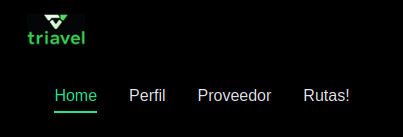
\includegraphics[width=0.7\textwidth]{Content/Images/ManualBarraNavegacion.png}
    \footnote{Nota. \textup{Fuente : Autores.}}
    \end{minipage}



La barra de busqueda permite a los usuarios encontrar rutas, destinos o proveedores de manera rápida y eficiente. Al escribir una palabra clave en la barra de búsqueda, el sistema sugiere resultados relevantes en tiempo real, facilitando la navegación y el acceso a la información deseada. Esta funcionalidad mejora significativamente la experiencia del usuario al reducir el tiempo necesario para localizar opciones específicas dentro de la aplicación.

     \vspace{2mm}
    \begin{minipage}{0.9\textwidth}
    \centering
    \captionof{figure}[{Barra de Busqueda.}]{Barra de Busqueda.}
    \label{ManualBarraNavegacion}
    
\includegraphics[width=0.7\textwidth]{Content/Images/ManualBarraBusqueda.png}
    \footnote{Nota. \textup{Fuente : Autores.}}
    \end{minipage}


    Los botones principales de busqueda para filtrar los Restaurantes, hoteles y demás sitios turísticos ayudan a filtrar los espacios para que aparezcan de acuerdo a las necesidades del usuario.

      \vspace{2mm}
    \begin{minipage}{0.9\textwidth}
    \centering
    \captionof{figure}[{Botones de busqueda.}]{Botones de busqueda.}
    \label{ManualBarraNavegacion}
    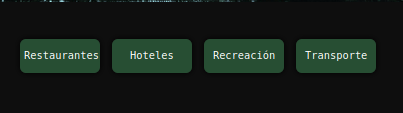
\includegraphics[width=0.7\textwidth]{Content/Images/ManualBotonesDeBusqueda.png}
    \footnote{Nota. \textup{Fuente : Autores.}}
    \end{minipage}

    Los botones de carrusel permiten el desplazamiento entre los diferentes elementos dispuestos entre carruseles, sean lugares, noticias o reseñas.

      \vspace{2mm}
    \begin{minipage}{0.9\textwidth}
    \centering
    \captionof{figure}[{Botones de busqueda.}]{Botones de busqueda.}
    \label{ManualBarraNavegacion}
    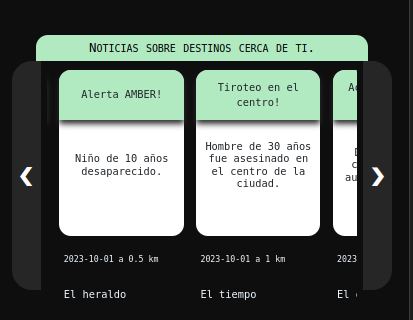
\includegraphics[width=0.7\textwidth]{Content/Images/ManualFlechasCarrusel.png}
    \footnote{Nota. \textup{Fuente : Autores.}}
    \end{minipage}

    .


\end{document}